\documentclass[12pt]{article}
\usepackage{amsmath,amssymb,amsthm}
\usepackage[english]{babel}
\usepackage[utf8]{inputenc}
\usepackage{fancyhdr}
\usepackage{changepage} 

% for line spacing
\usepackage{setspace}

% for absolute value
\usepackage{commath}

% for numbering
\usepackage{enumerate}

% for image placing
\usepackage{float}

% paper size and margins
\usepackage[letterpaper, left=20mm, right=20mm, top=25mm, bottom = 25mm, headsep=.15in]{geometry}

% for curly brace
\usepackage{amsmath}

% for input images
\usepackage{graphicx}
\graphicspath{ {./} }
\usepackage{subfig}

% for printing pseudocode
\usepackage[boxed]{algorithm}
\usepackage[noend]{algpseudocode}

% for tables
\usepackage{tabularx}

\makeatletter
\def\BState{\State\hskip-\ALG@thistlm}
\makeatother

% for circled numbers
\usepackage{tikz}
\newcommand*\circled[1]{\tikz[baseline=(char.base)]{
            \node[shape=circle,draw,inner sep=1pt] (char) {#1};}}

% double line space
\renewcommand{\baselinestretch}{2.0}

% header, footer and page number
\pagestyle{fancy}
\fancyhf{}
\rhead{Tiankai Jiang \quad 20834939}
\lhead{ECE657A \quad Assignment 2}
\fancyfoot[C]{\thepage}

\setlength{\headheight}{15pt}

\begin{document}
\noindent
{\LARGE The source code is at the end of this document}\\
\textbf{\large Question 1:}\\
\textbf{Normalization}
\begin{center}
    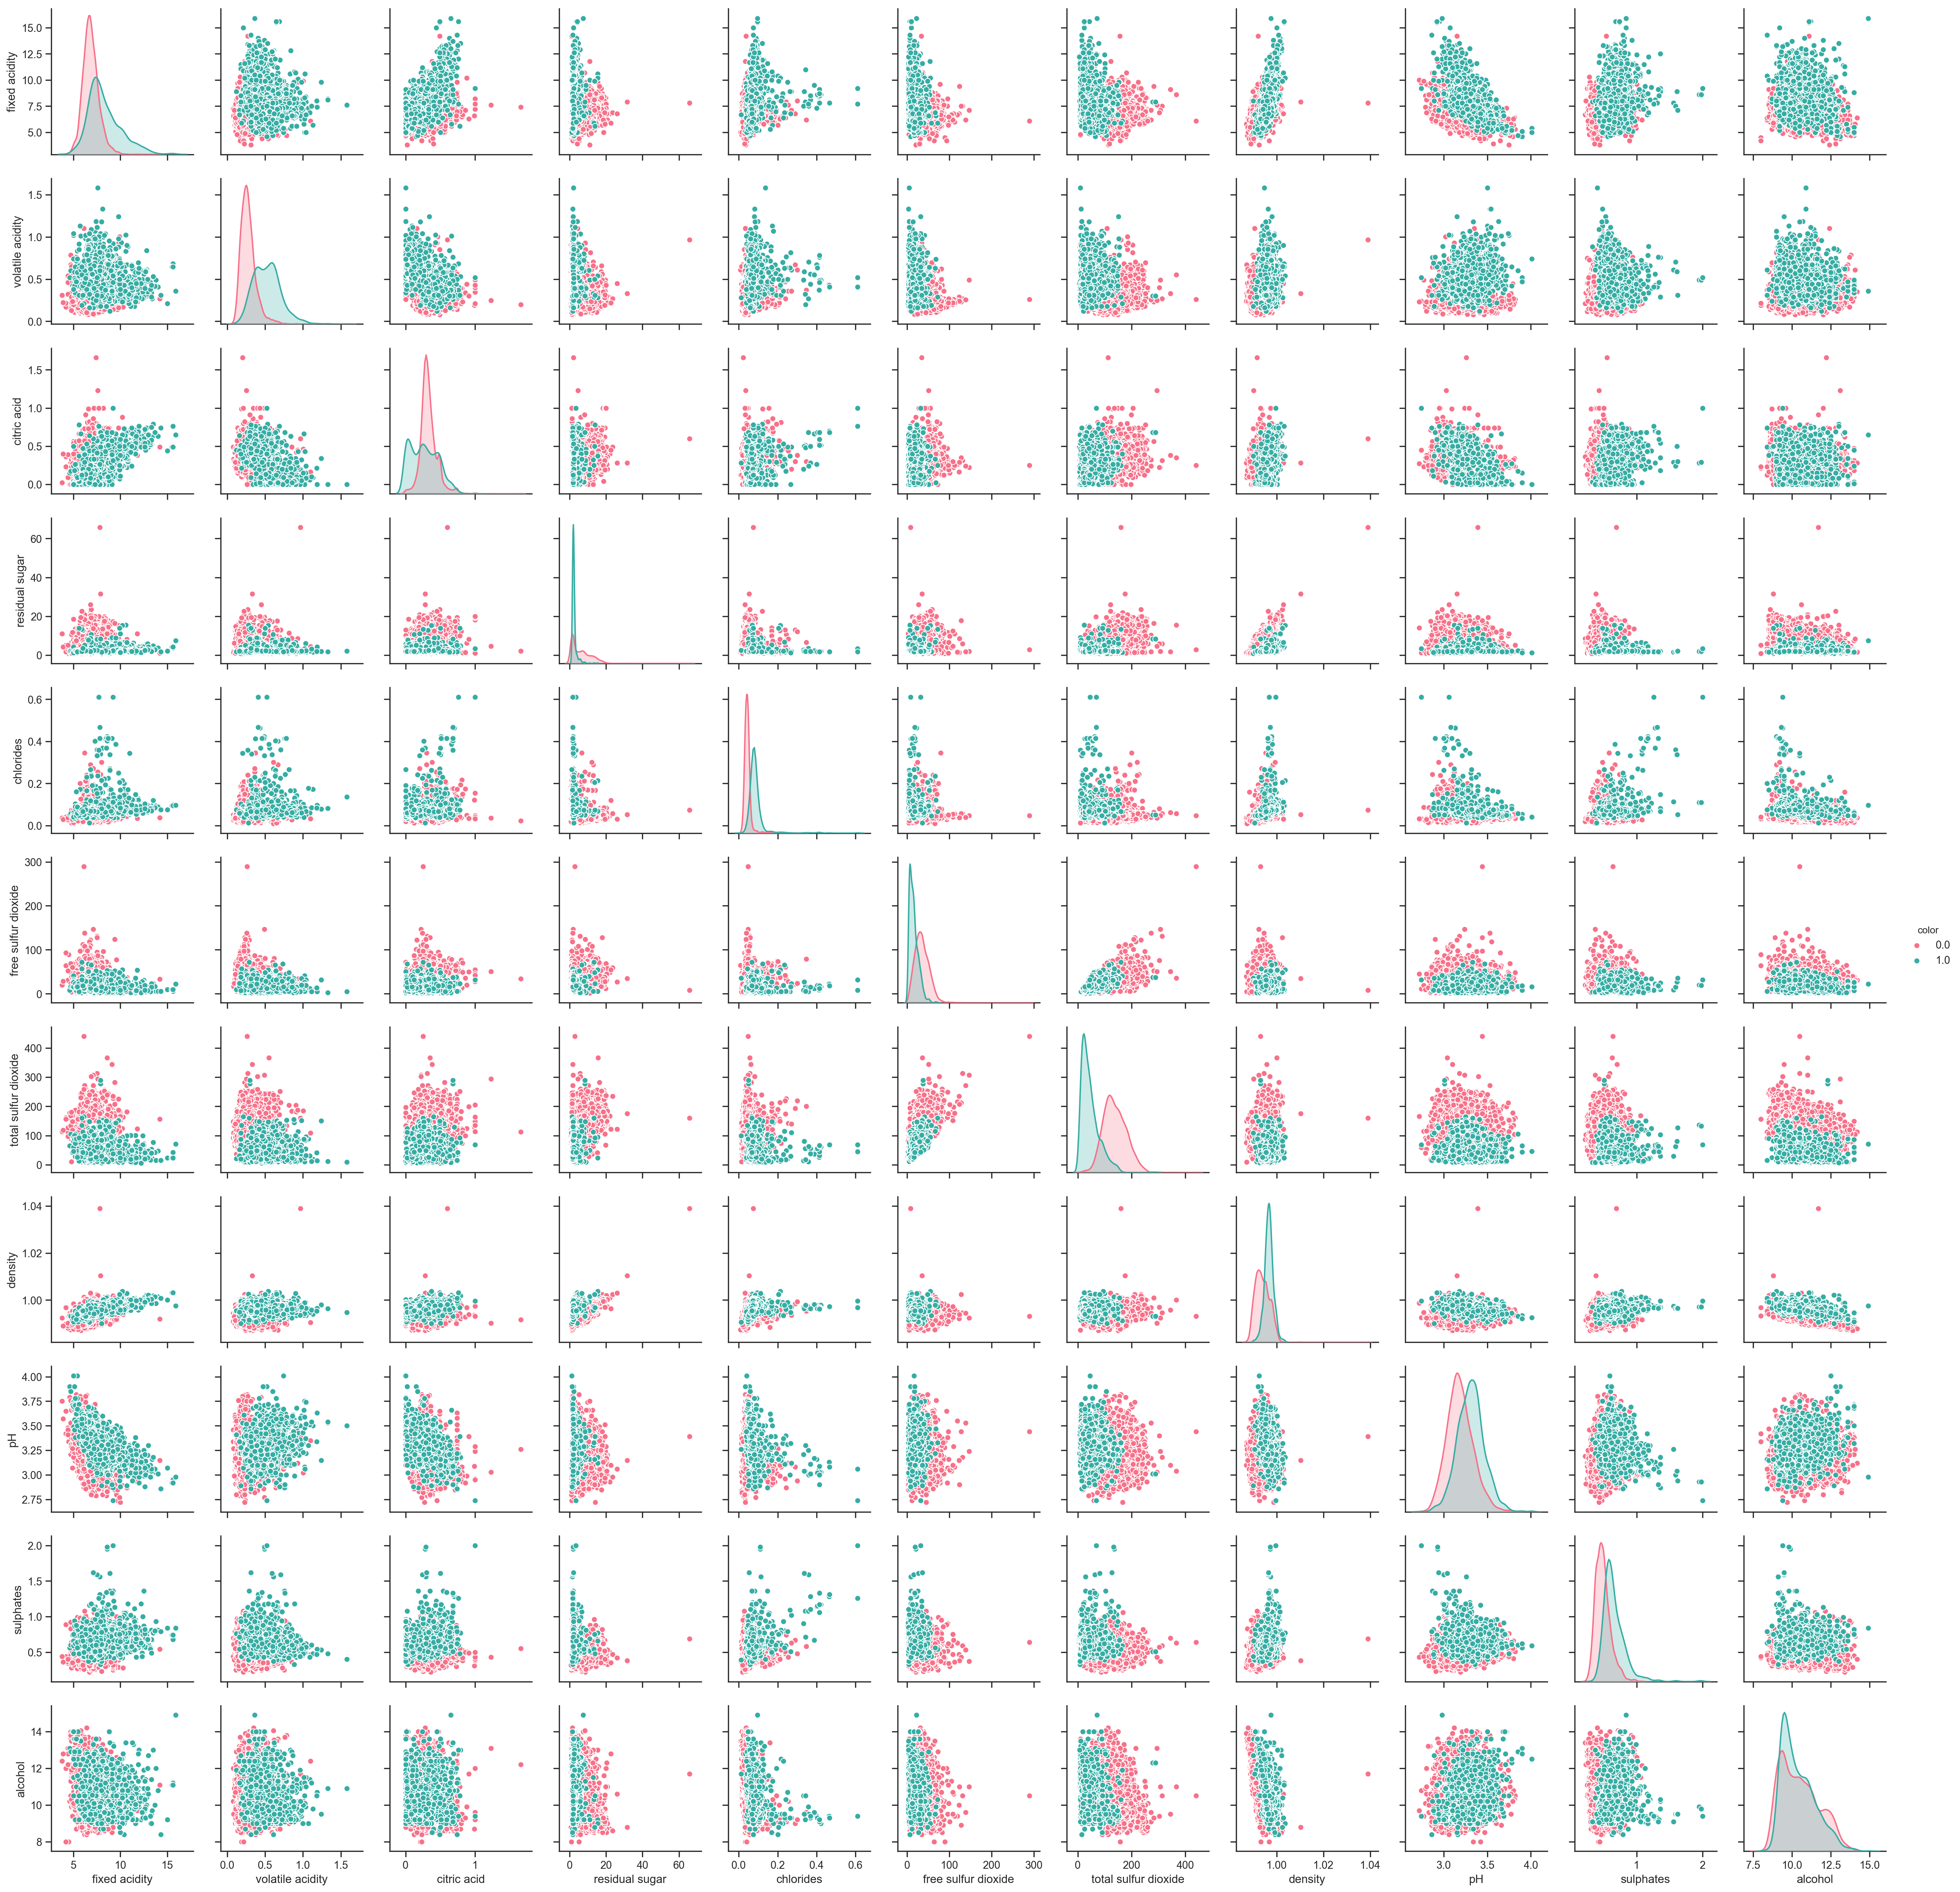
\includegraphics[width=17cm]{../plots/Q1_no_normalization.png}
    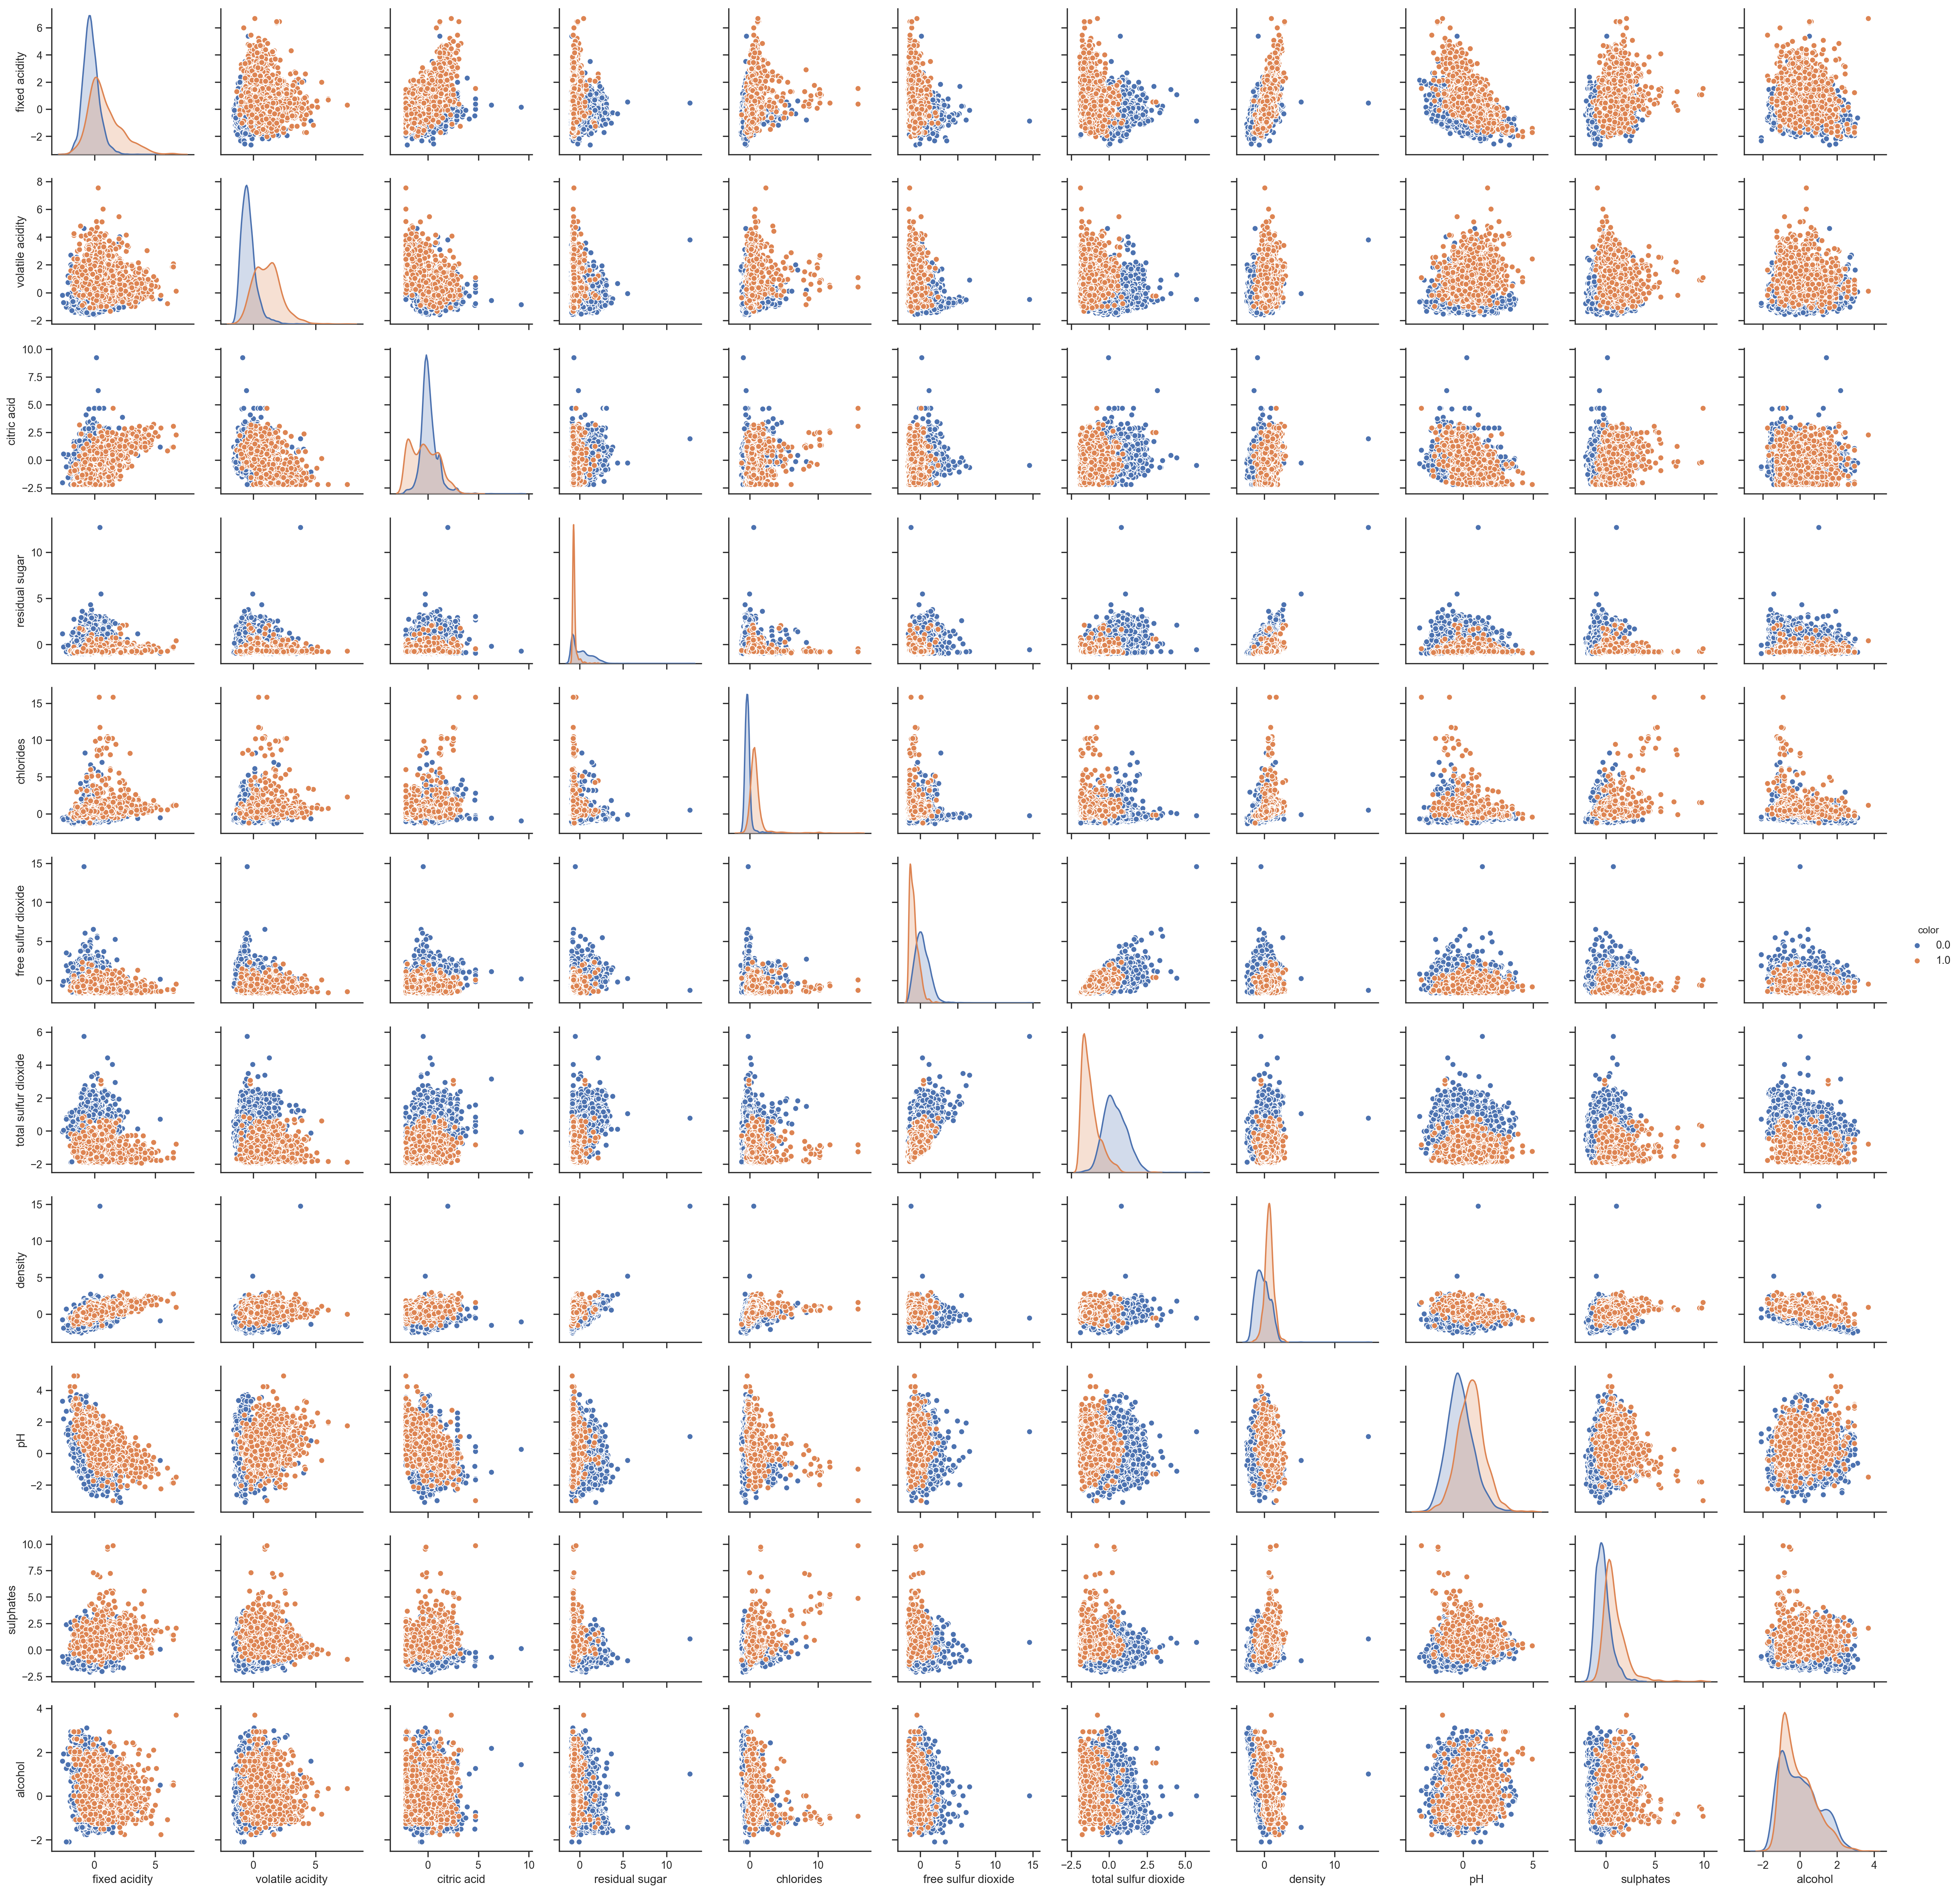
\includegraphics[width=17cm]{../plots/Q1_zscore_normalization.png}
\end{center}
\noindent
The first graph is plotted without normalization and the second is plotted after z-score normalization. Points in both plots have the same distribution. However, the range of the axes of the unnormalized plot varies with each feature, but that of the normalized plot are all the same -- the majority of points scattered between -2 to 5 on both axes, with a mean of zero.\\\\\\
\textbf{KNN Classification With All Features}
\begin{figure}[H]
\captionsetup[subfigure]{labelformat=empty}
\centering
\subfloat[]{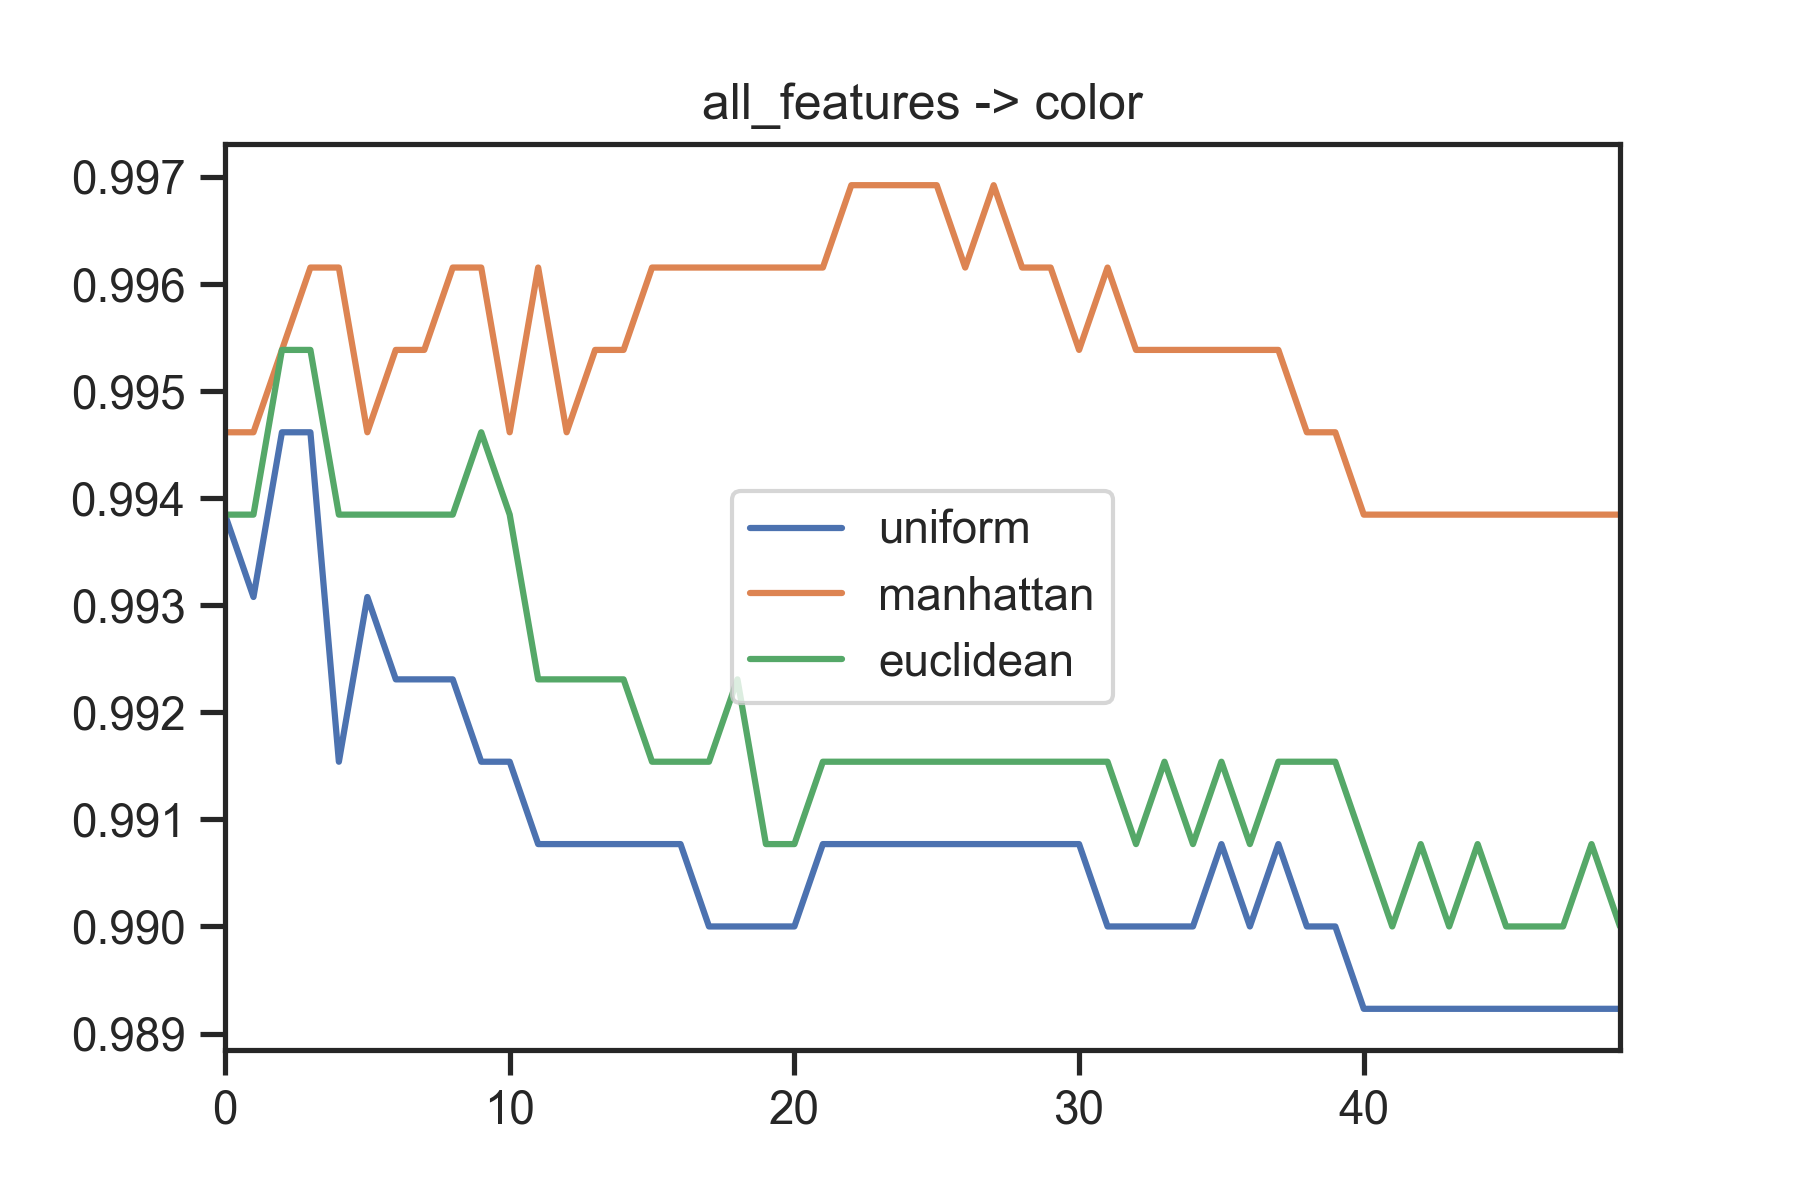
\includegraphics[width=0.48\textwidth]{../plots/Q1_all_features_color.png}}
\subfloat[] {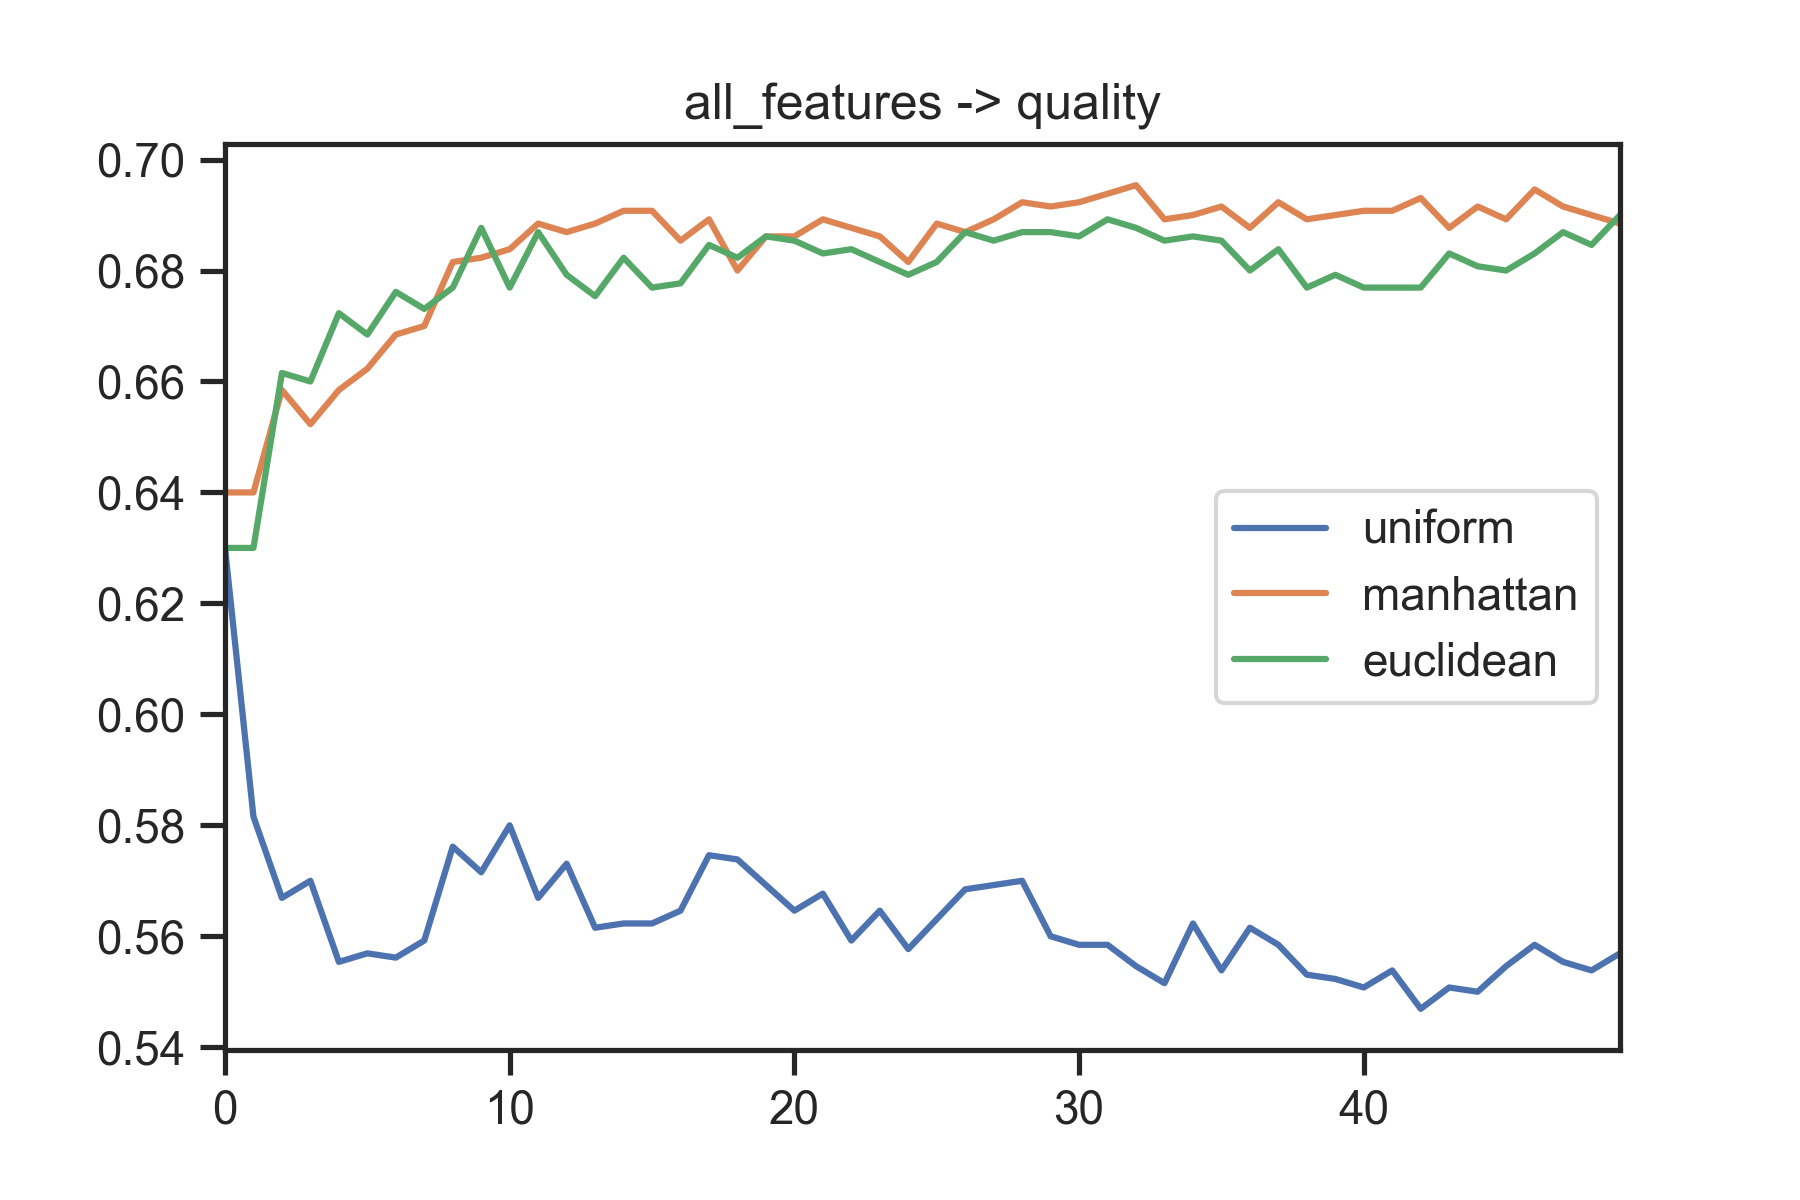
\includegraphics[width=0.48\textwidth]{../plots/Q1_all_features_quality.png}}
\end{figure}
\noindent
\textbf{Bonus: KNN Classification With Better Schemes}\\
It is rather difficult to find knn parameters that are better than manhattan distance. But we can find a preprocessing scaler that is better than z-normalization. For quality, using PowerTransformer is better than using z-norm. And for quality prediction, using RobustScaler or OrdinalEncoder will produce a better result when $k>33$. The code is at the end of the jupyter notebook and commented out since it takes about 3 minutes to run.
\begin{figure}[H]
\captionsetup[subfigure]{labelformat=empty}
\centering
\subfloat[]{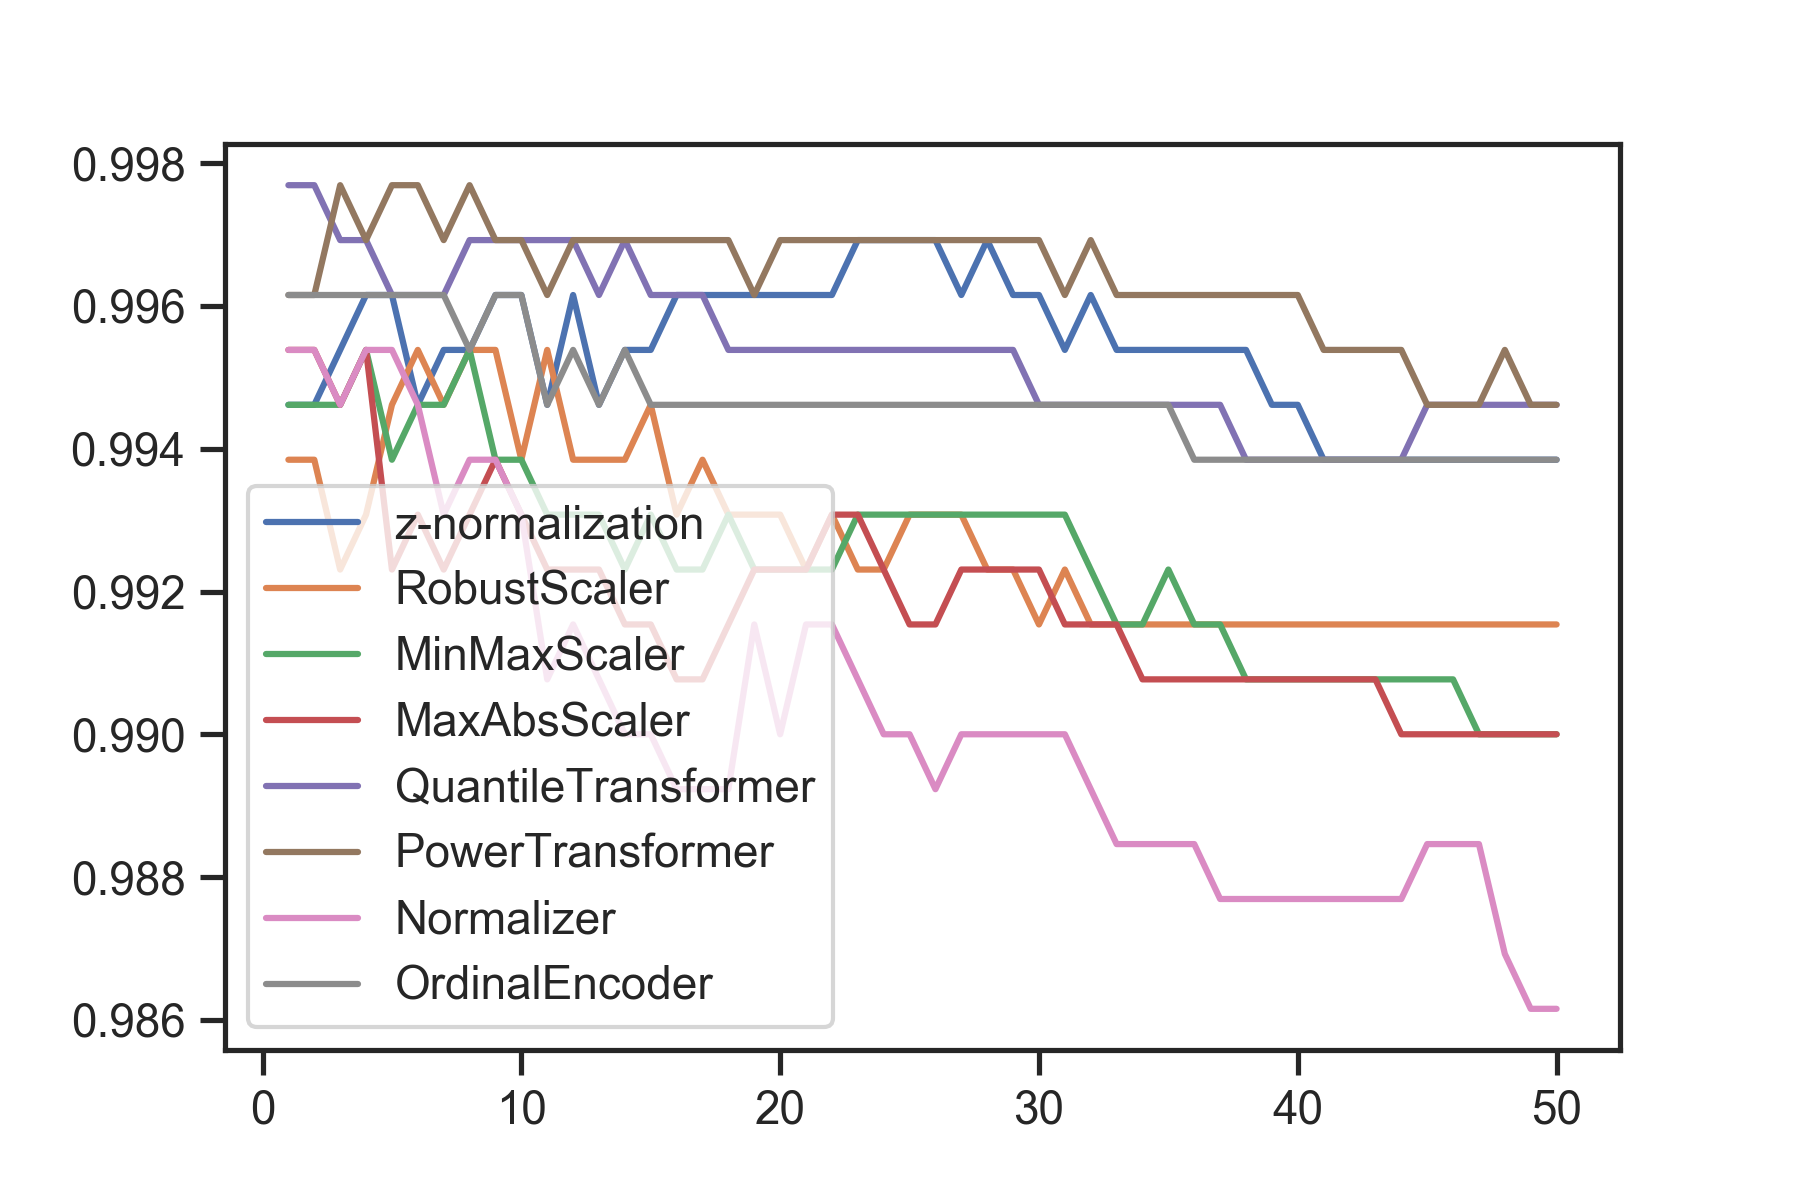
\includegraphics[width=0.48\textwidth]{../plots/Q1_BestParam_color.png}}
\subfloat[] {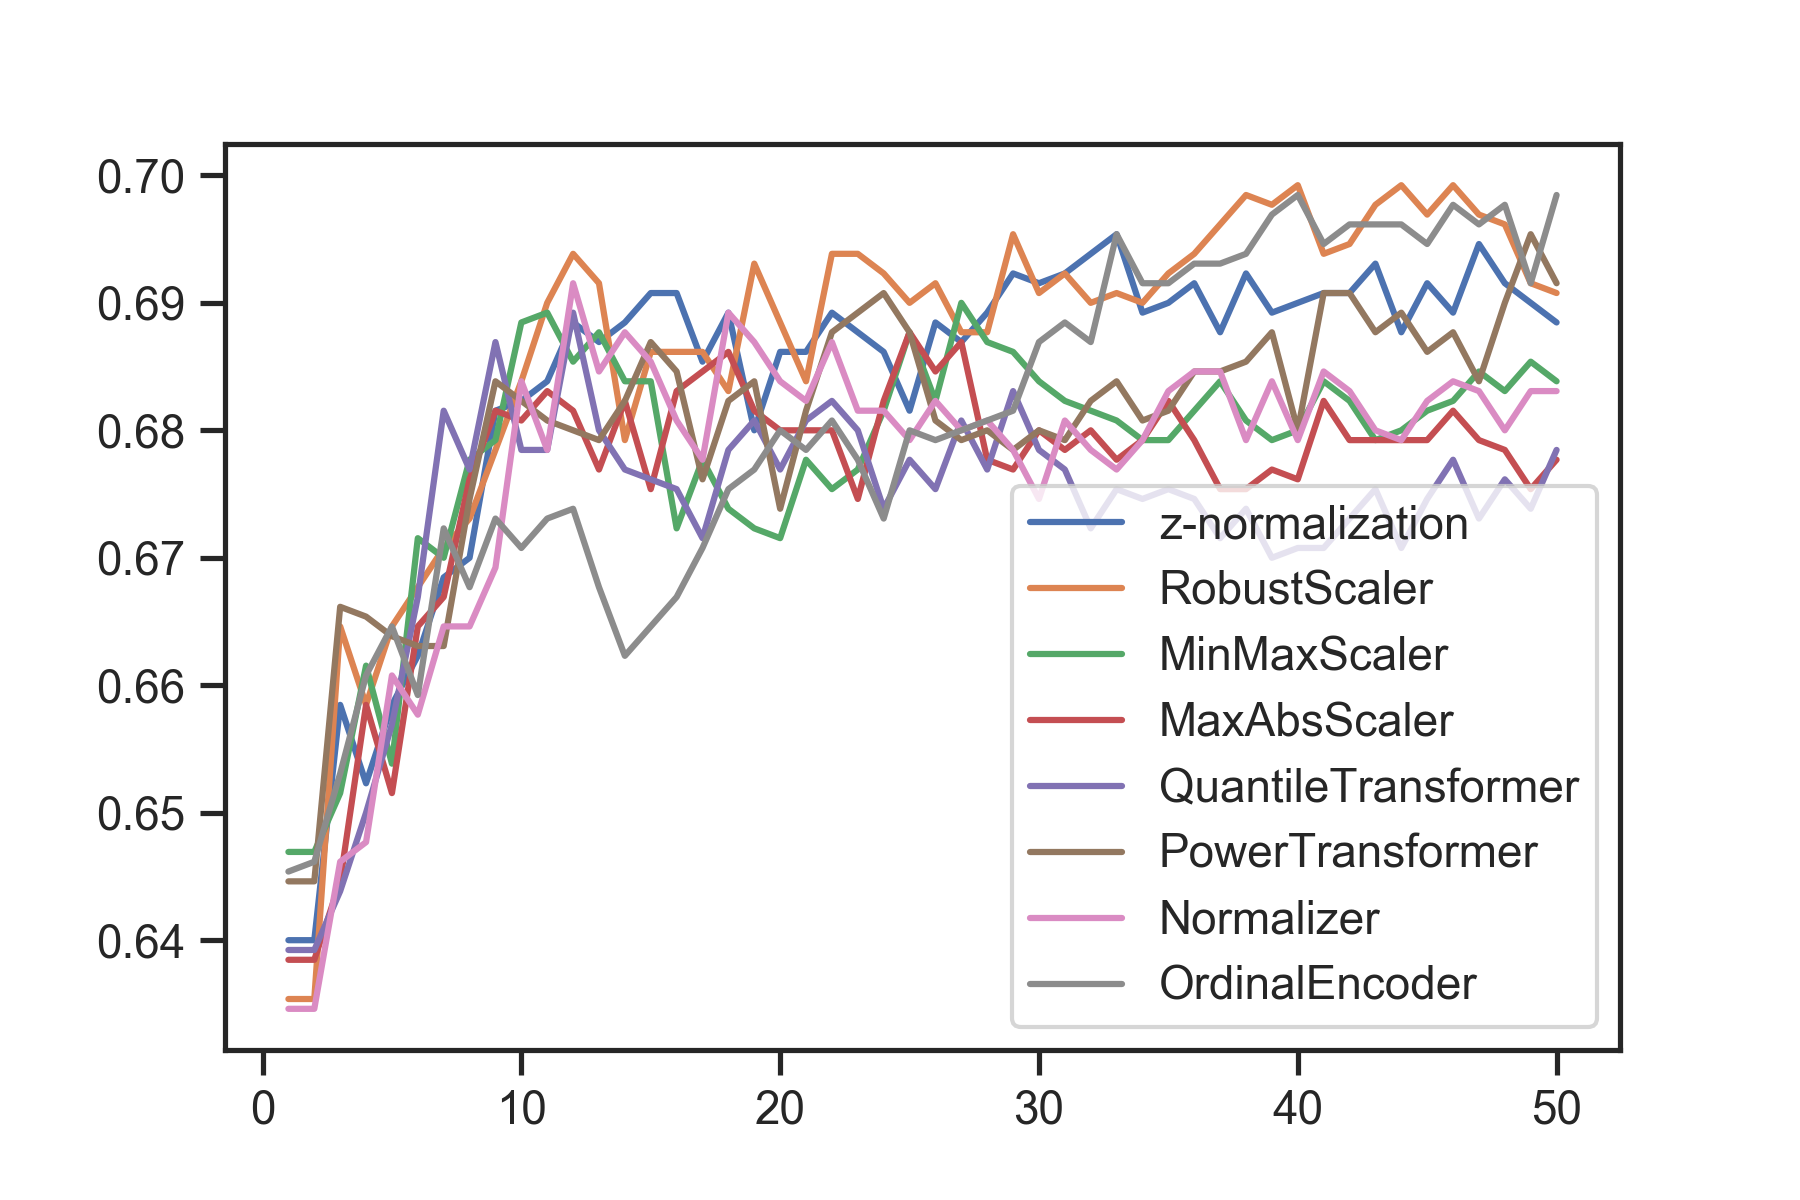
\includegraphics[width=0.48\textwidth]{../plots/Q1_BestParam_quality.png}}
\end{figure}
\noindent
\textbf{Bonus: KNN Classification With Selected 4 Features}\\
Try all ${11 \choose 4}$ feature combinations and choose the best result. The code is at the end of the jupyter notebook and commented out since it takes about 30 minutes to run.\\
For color prediction under manhattan, no combination of 4 is better than using all features.\\
For color prediction under euclidean, using 'residual sugar', 'total sulfur dioxide', 'density', 'alcohol' yields the best result.
\begin{center}
    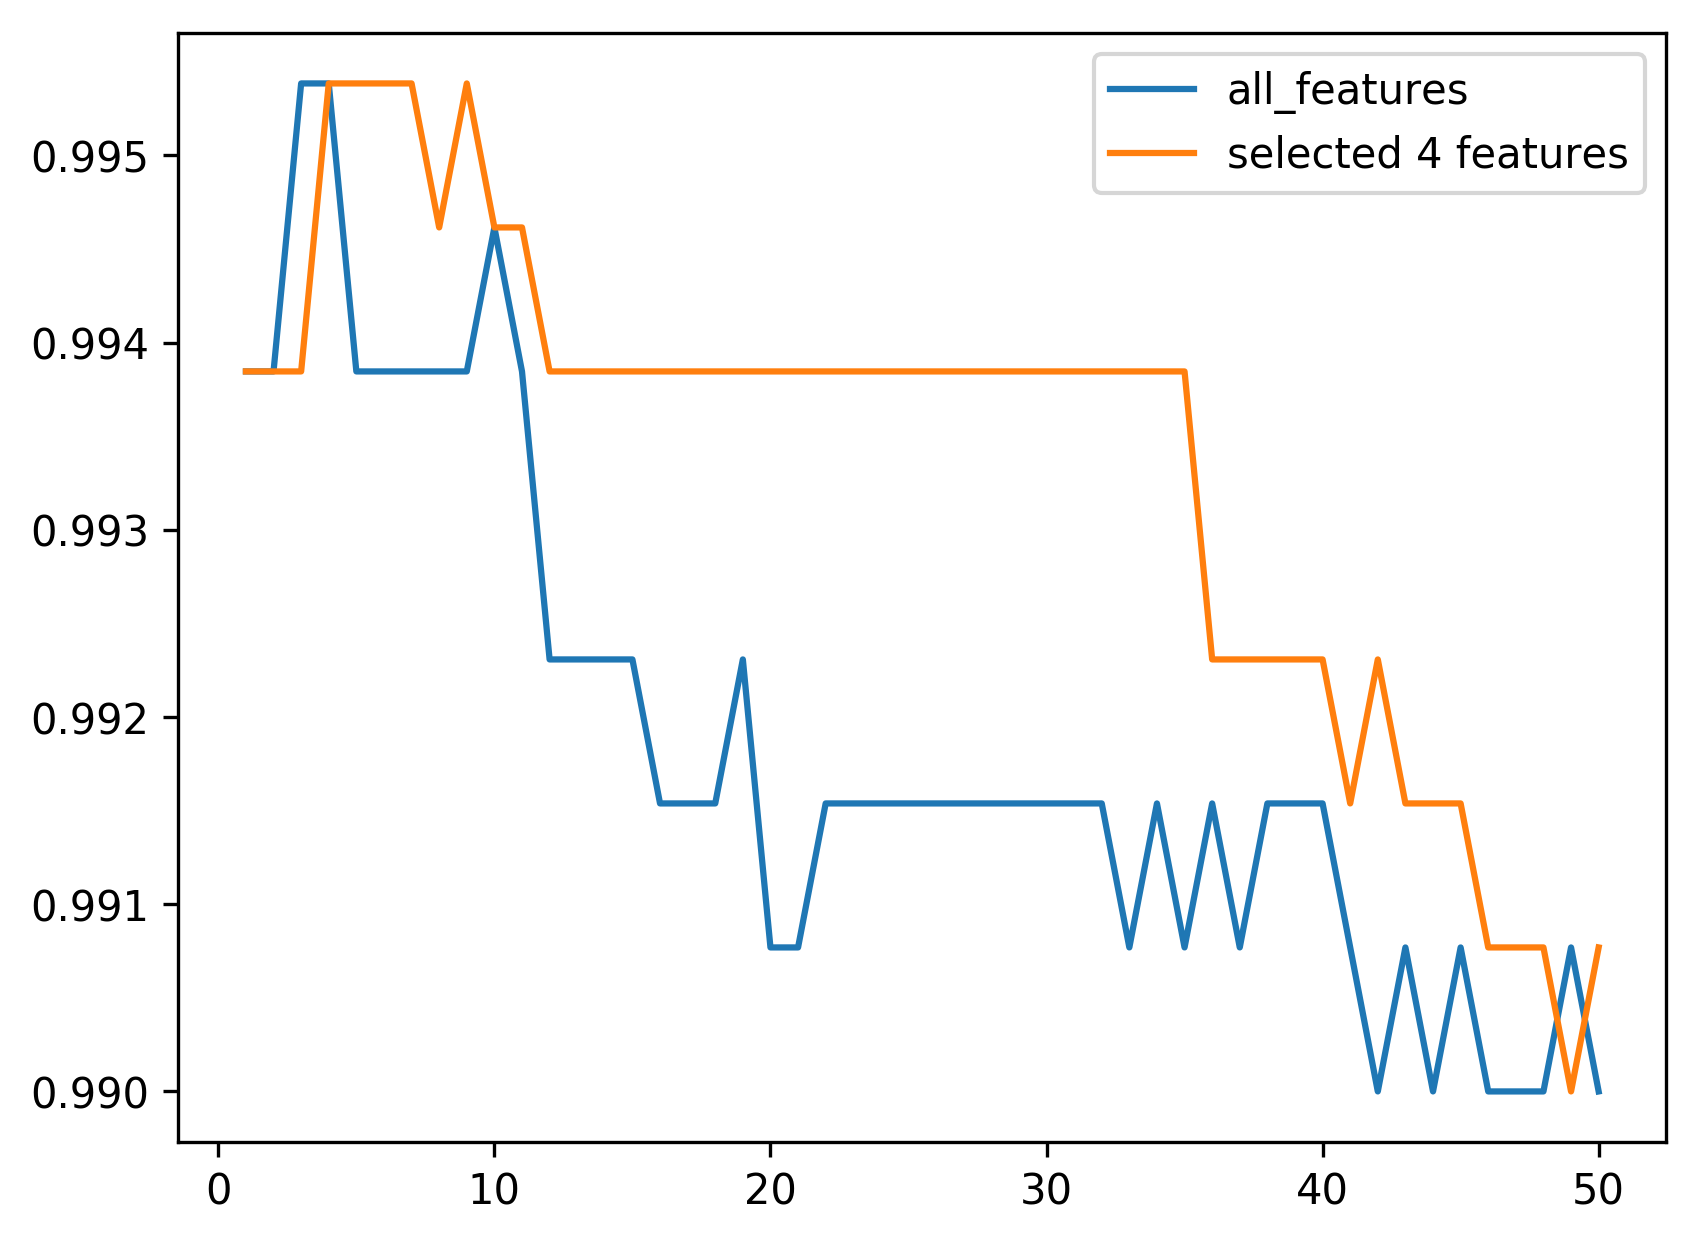
\includegraphics[width=9cm]{../select4features/color_e.png}
\end{center}
\noindent
For color prediction under uniform, using 'residual sugar', 'chlorides', 'total sulfur dioxide', 'density' yields the best result.
\begin{center}
    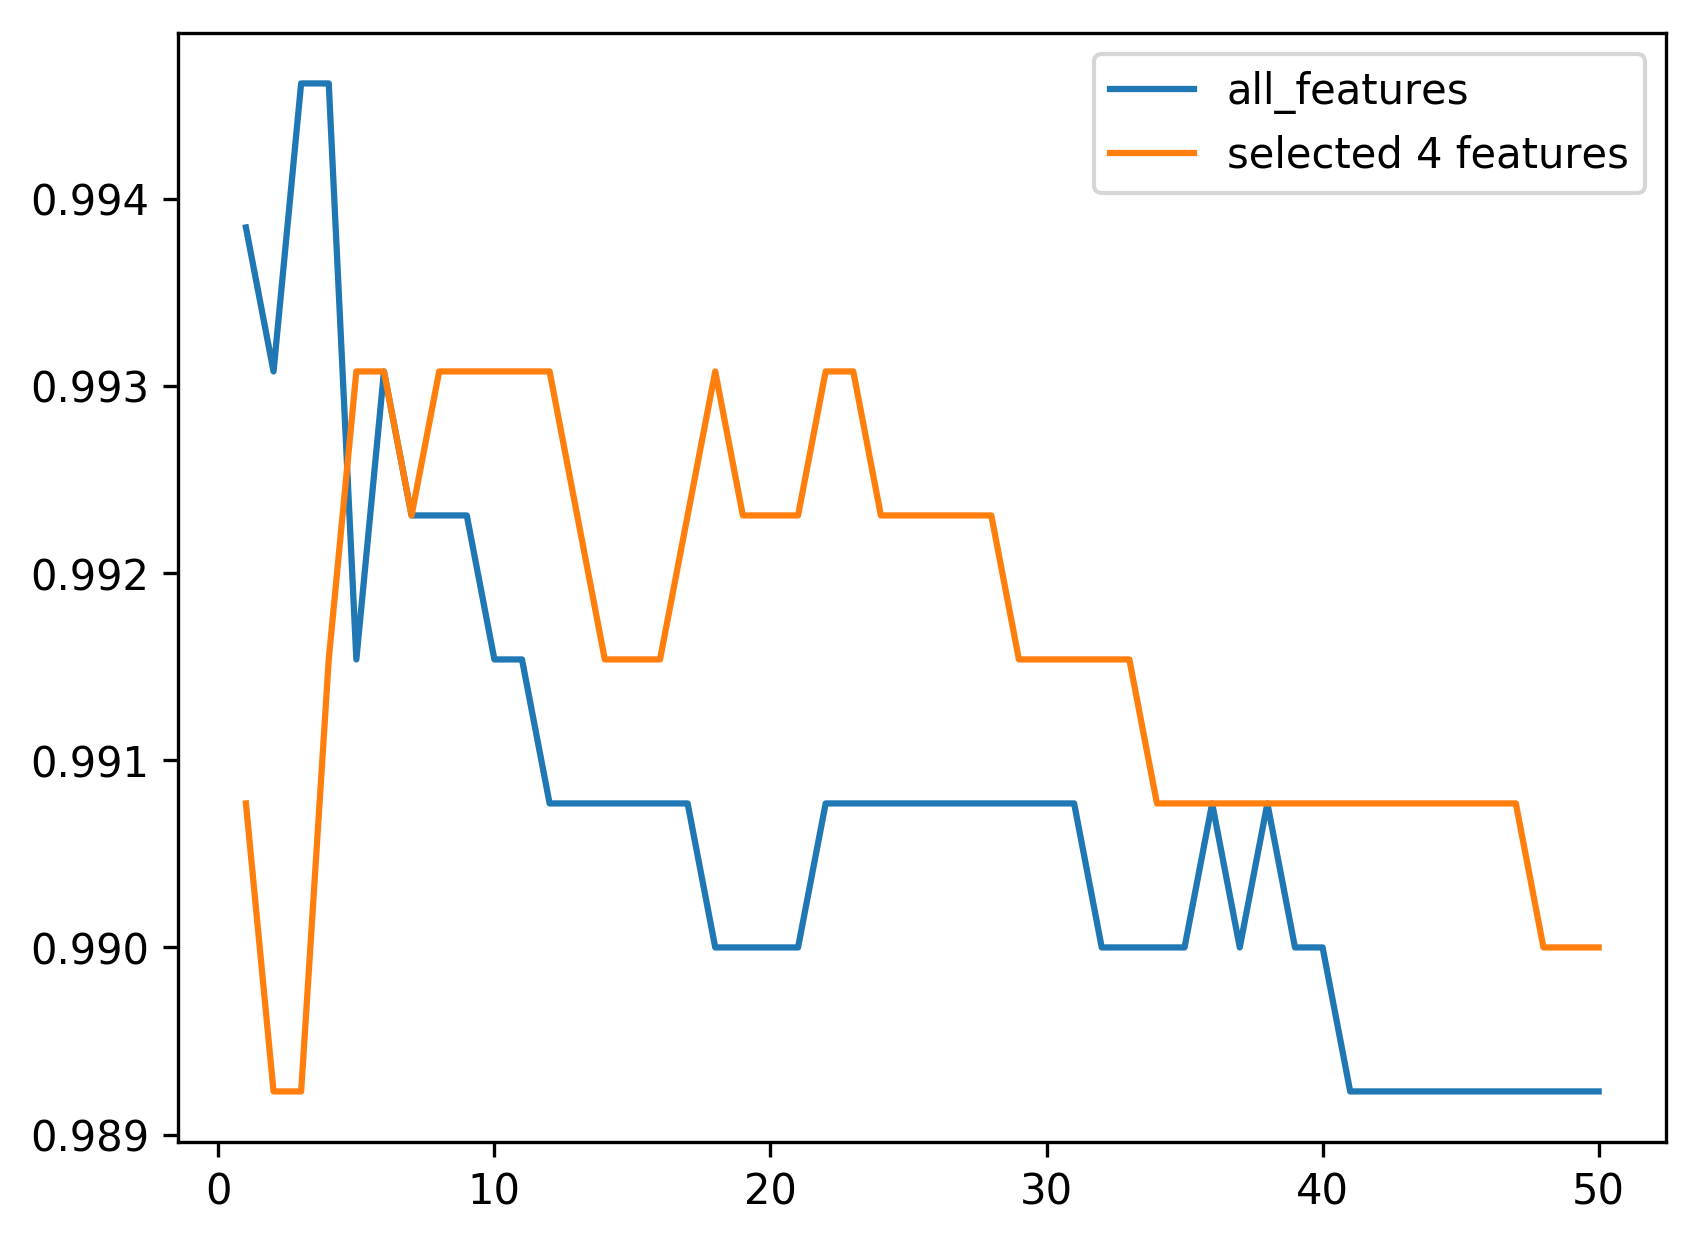
\includegraphics[width=9cm]{../select4features/color_u.png}
\end{center}
\noindent
For quality prediction under manhattan, no combination of 4 is better than using all features.\\
For quality prediction under euclidean, using 'volatile acidity', 'total sulfur dioxide', 'sulphates', 'alcohol' yields the best result.
\begin{center}
    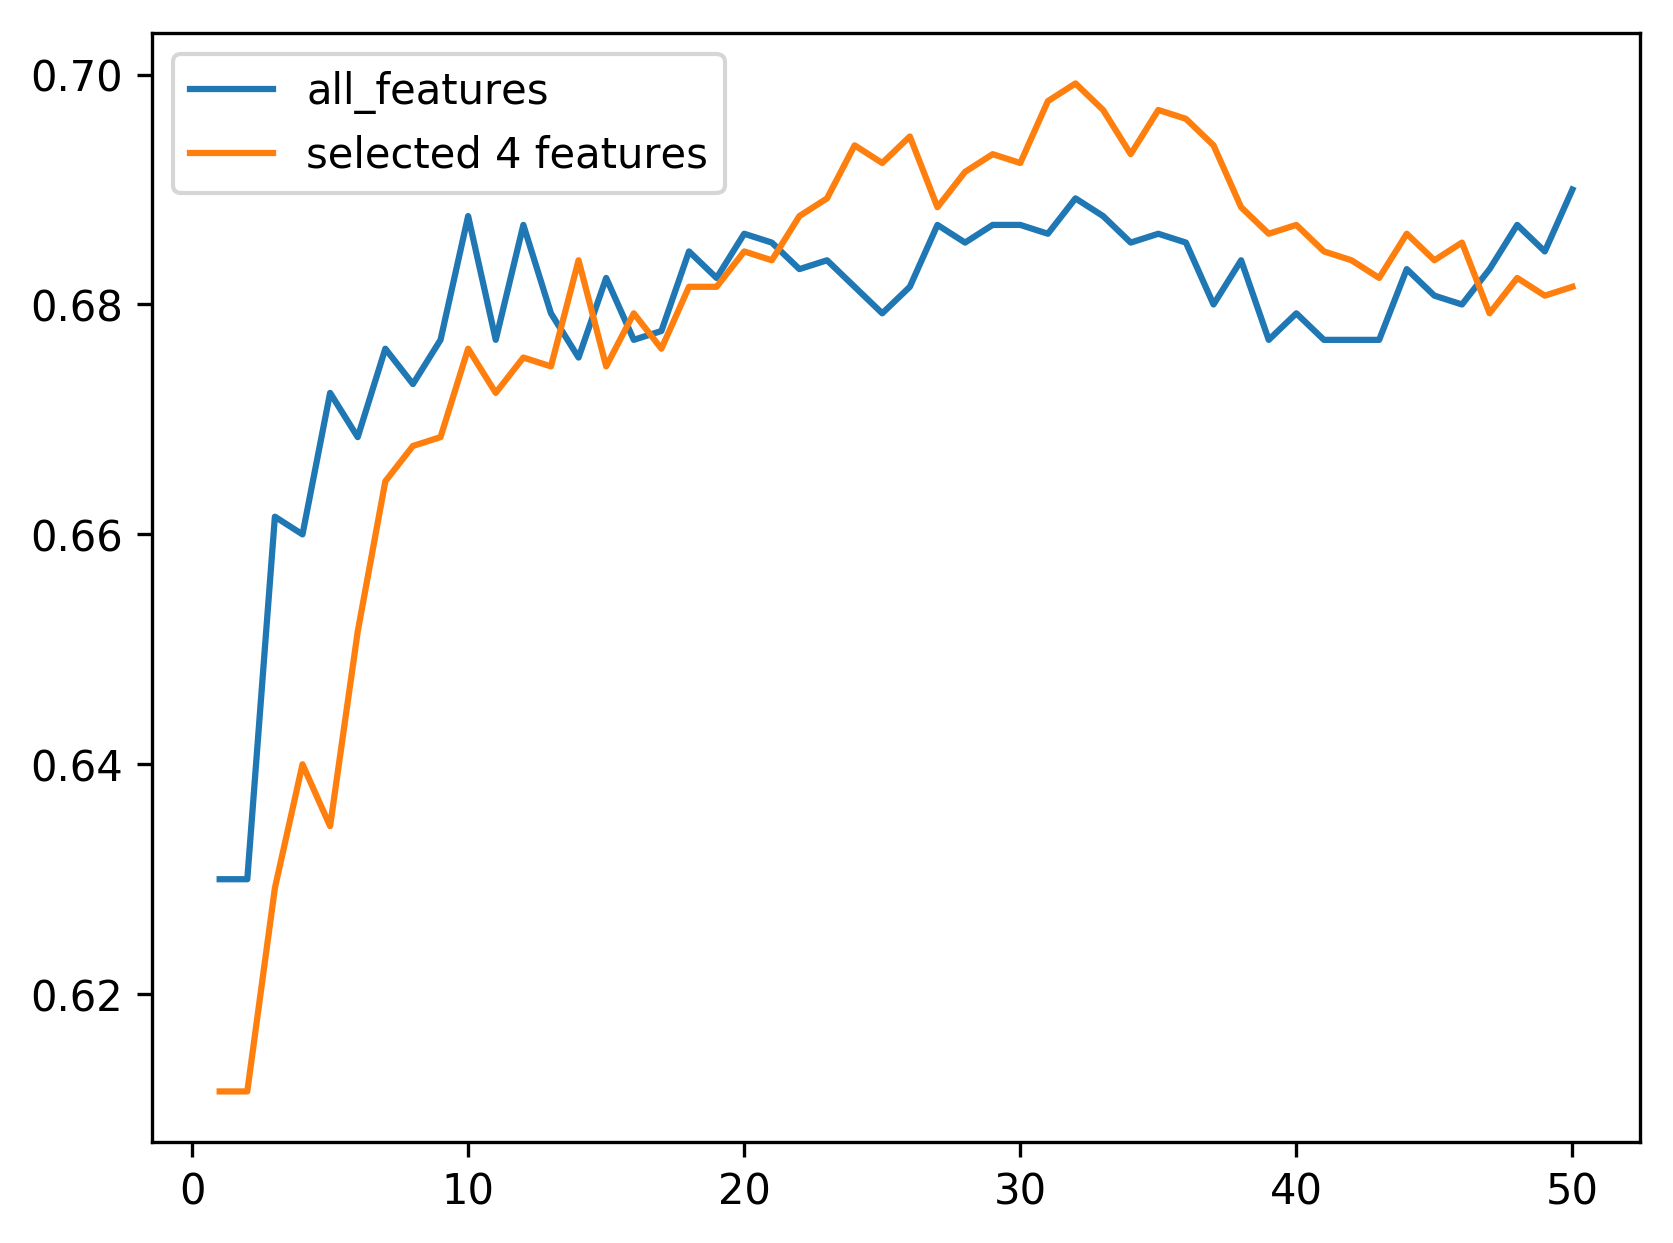
\includegraphics[width=9cm]{../select4features/quality_e.png}
\end{center}
\noindent
For quality prediction under uniform, using 'volatile acidity', 'total sulfur dioxide', 'density', 'alcohol' yields the best result.
\begin{center}
    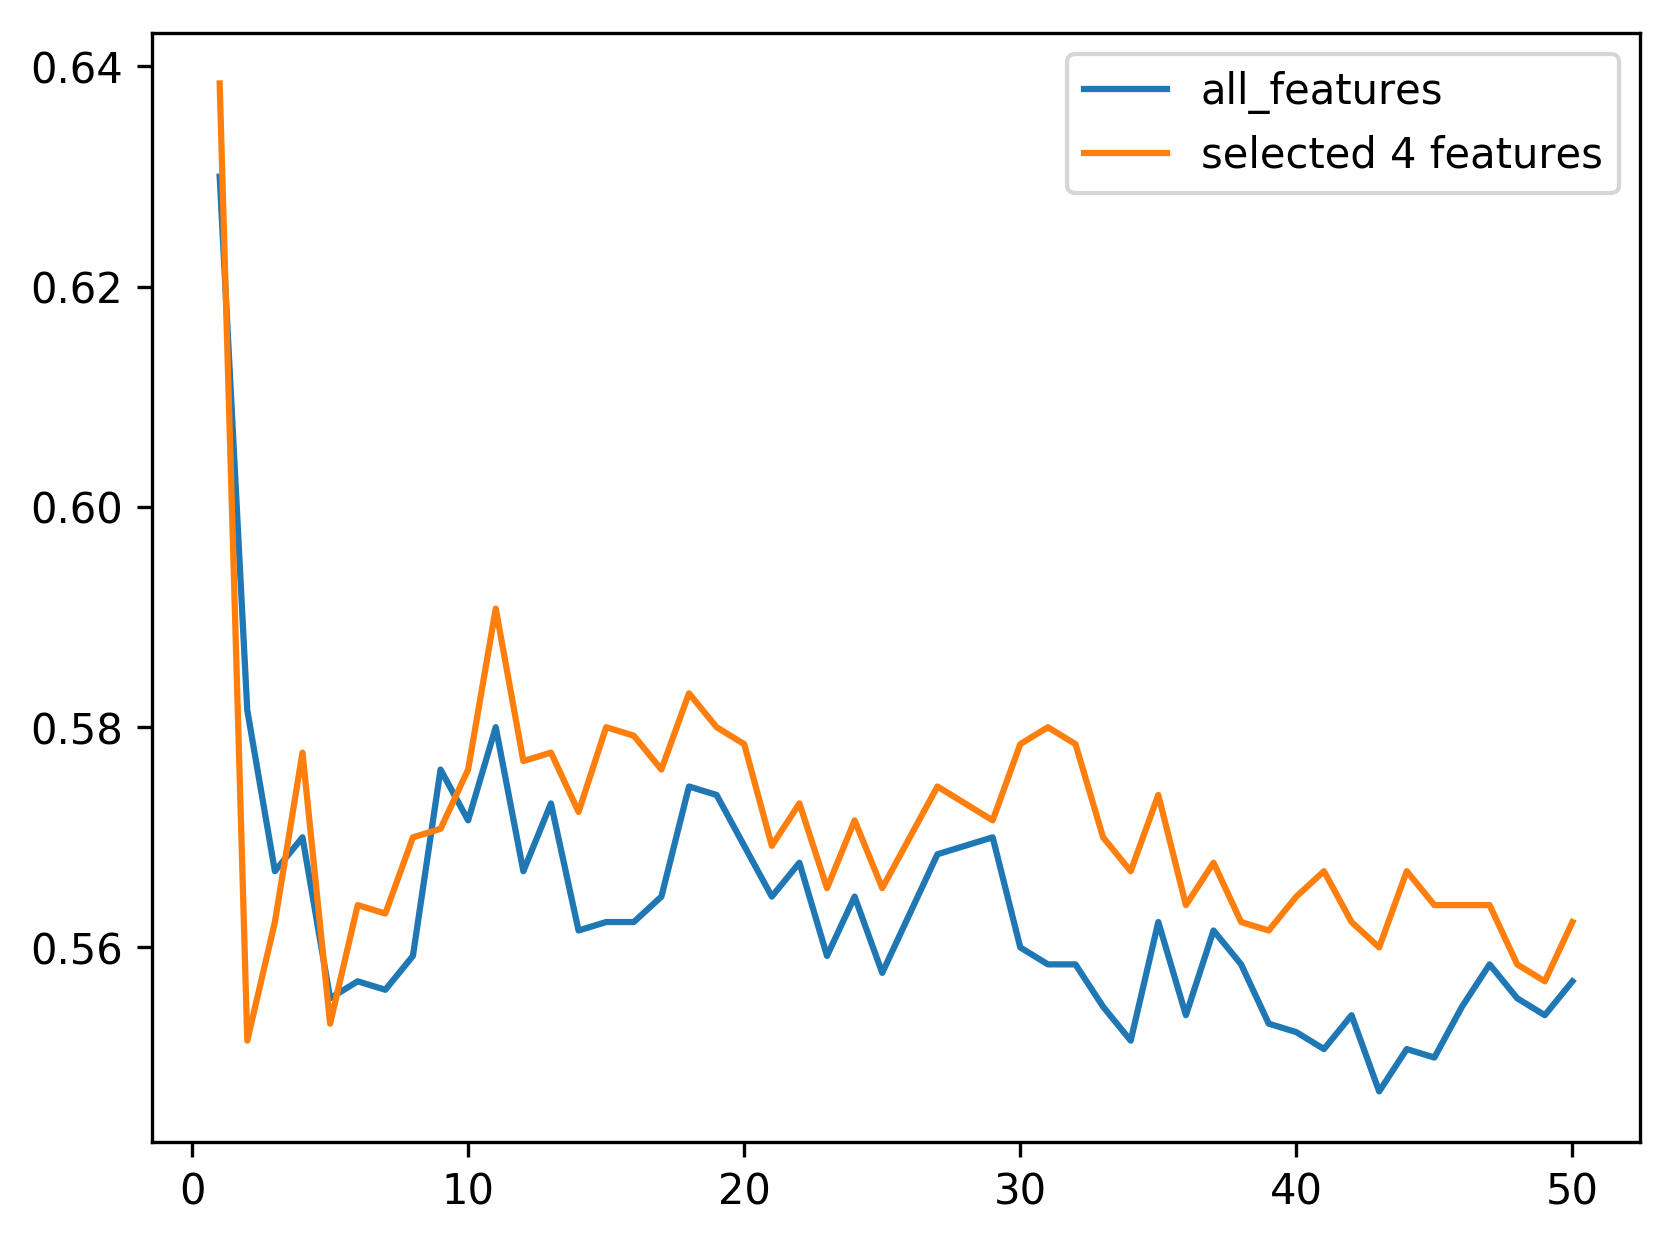
\includegraphics[width=9cm]{../select4features/quality_u.png}
\end{center}
\noindent
Because using all features for classification is better than using PCA or LDA, if the result of selected 4 features is better than using all features, it will for sure be better than using PCA or LDA.\\ For color prediction, using euclidean+['residual sugar', 'total sulfur dioxide', 'density', 'alcohol'] has a better result than PCA or LDA.\\
For quality prediction, using euclidean+['volatile acidity', 'total sulfur dioxide', 'sulphates', 'alcohol'] has a better result than PCA or LDA.\\\\\\
\textbf{KNN Classification With PCA Components}
\begin{figure}[H]
\captionsetup[subfigure]{labelformat=empty}
\centering
\subfloat[]{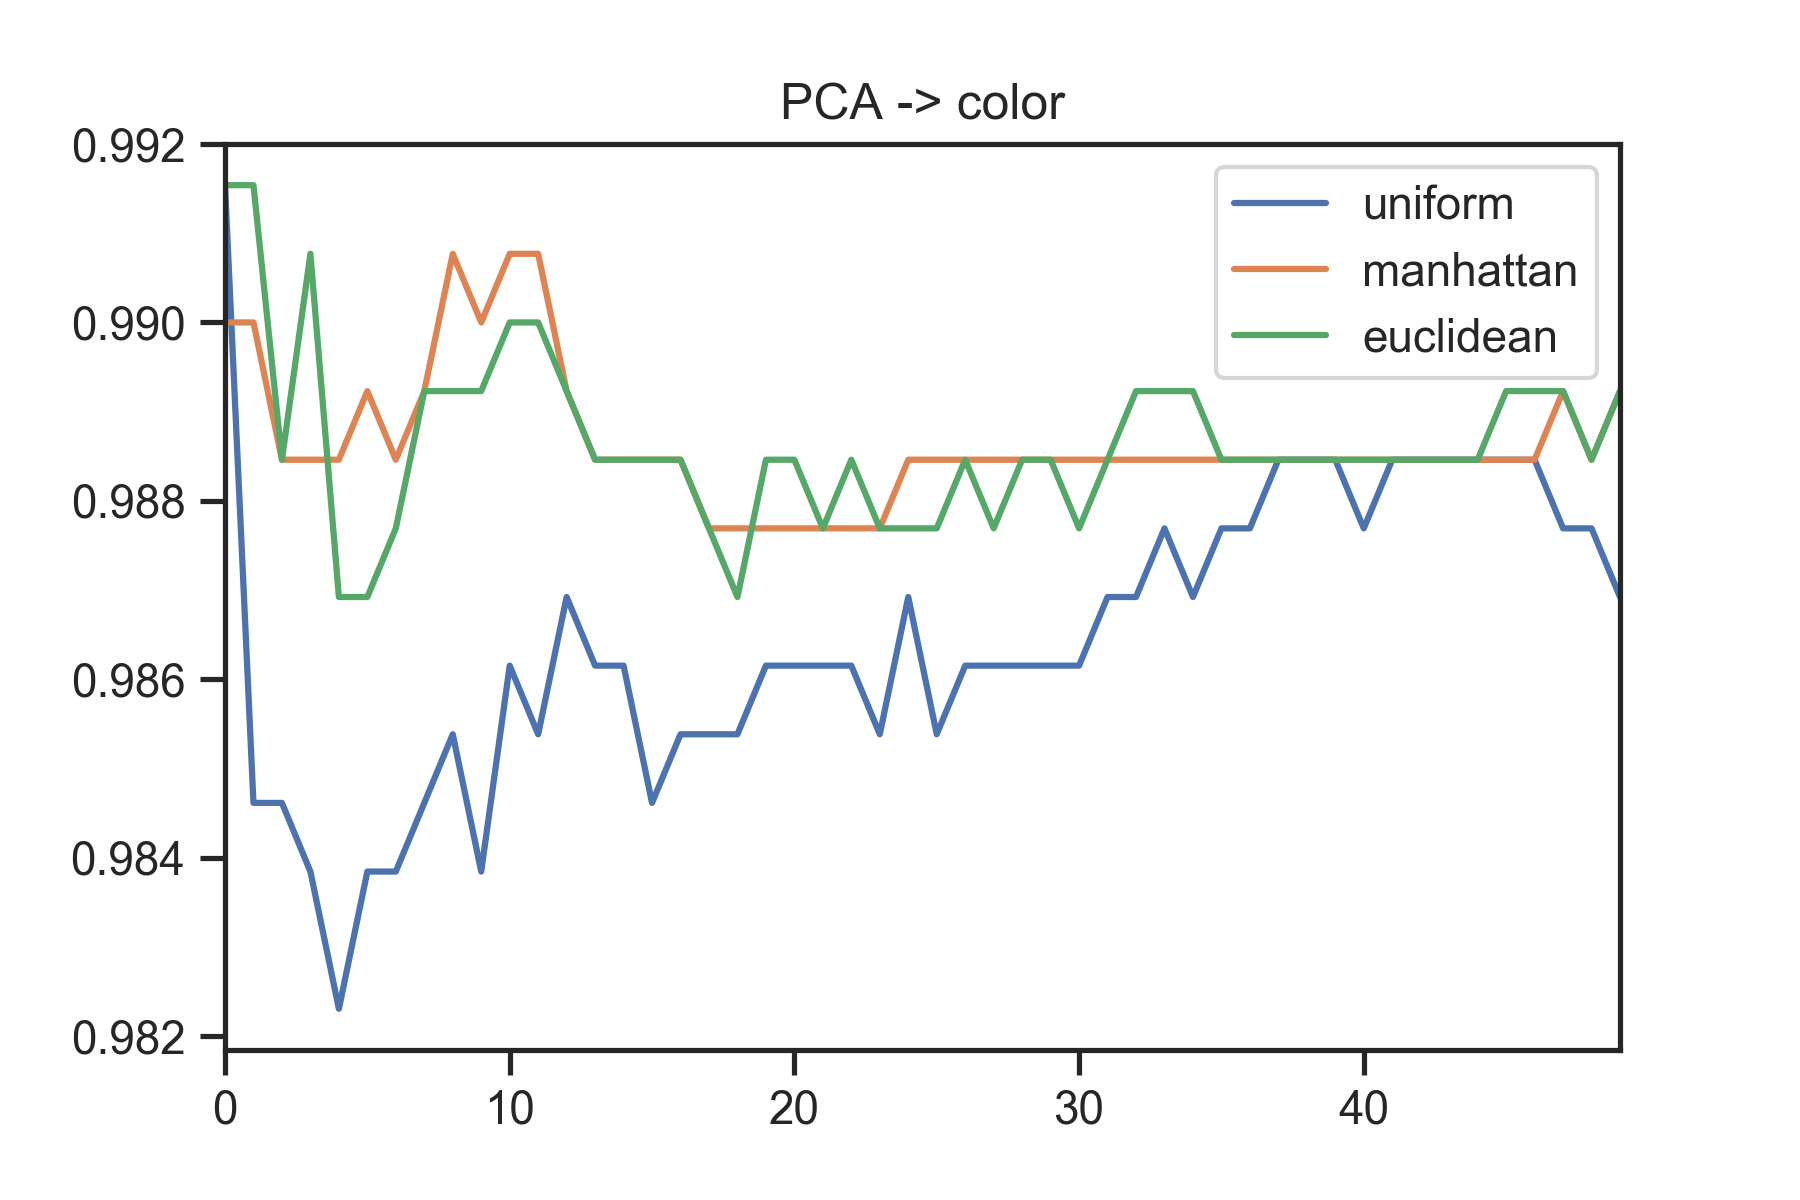
\includegraphics[width=0.48\textwidth]{../plots/Q1_PCA_color}}
\subfloat[] {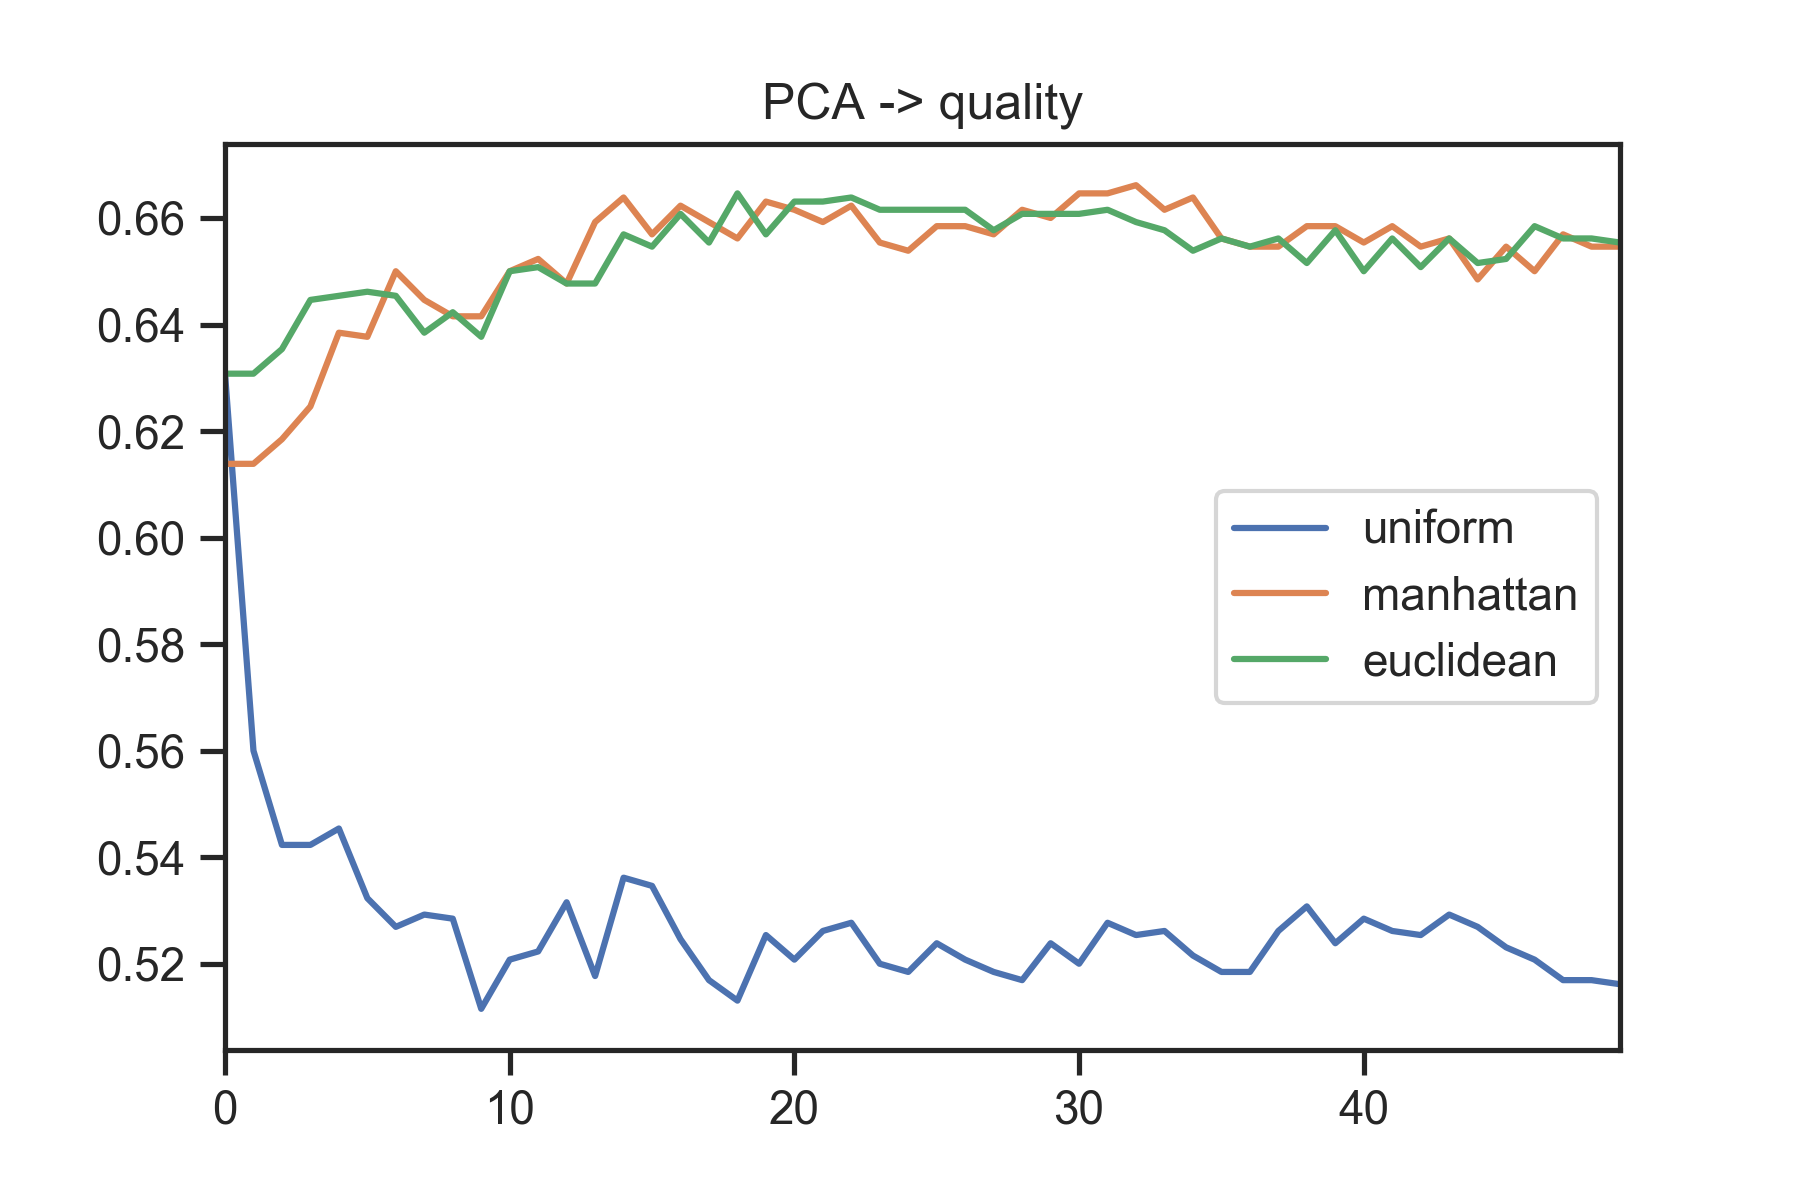
\includegraphics[width=0.48\textwidth]{../plots/Q1_PCA_quality.png}}
\end{figure}
\noindent
\textbf{KNN Classification With LDA Components}
\begin{figure}[H]
\captionsetup[subfigure]{labelformat=empty}
\centering
\subfloat[]{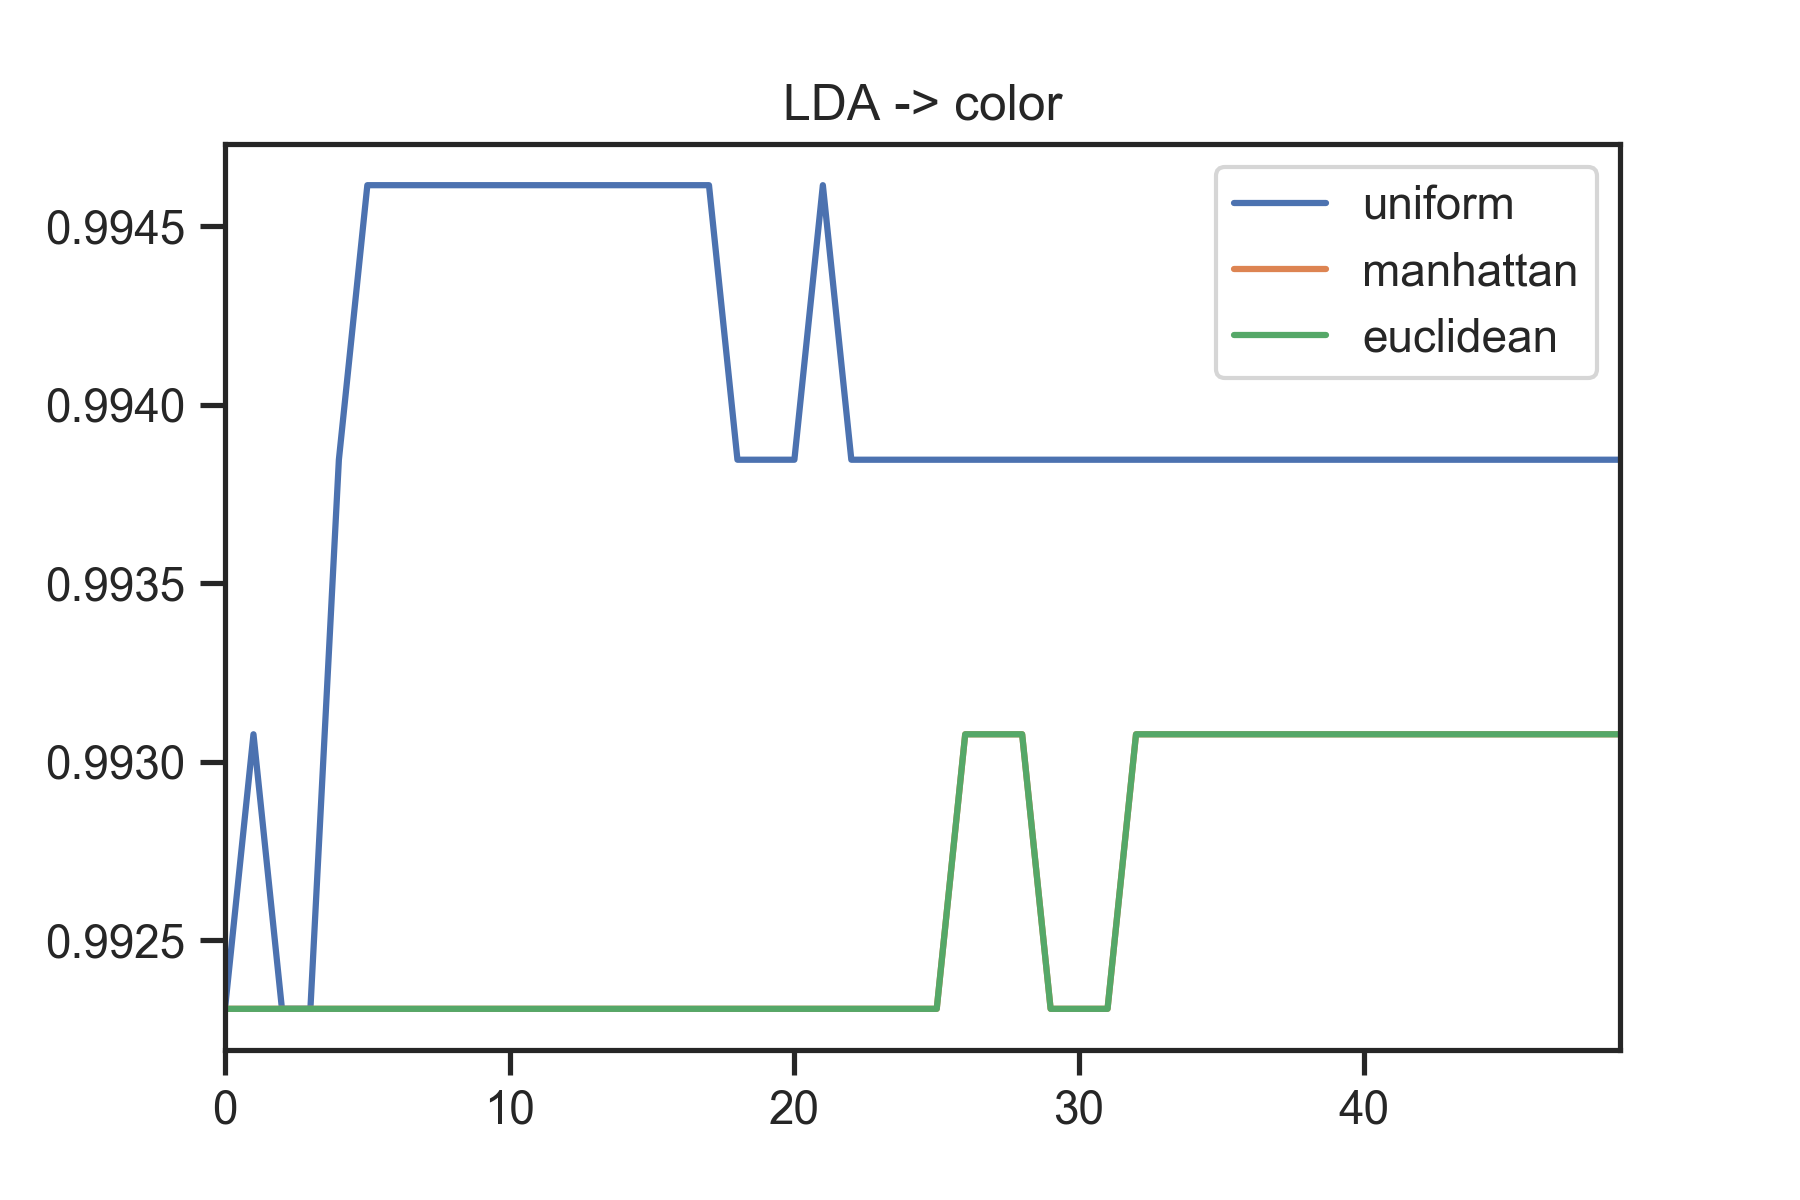
\includegraphics[width=0.48\textwidth]{../plots/Q1_LDA_color}}
\subfloat[] {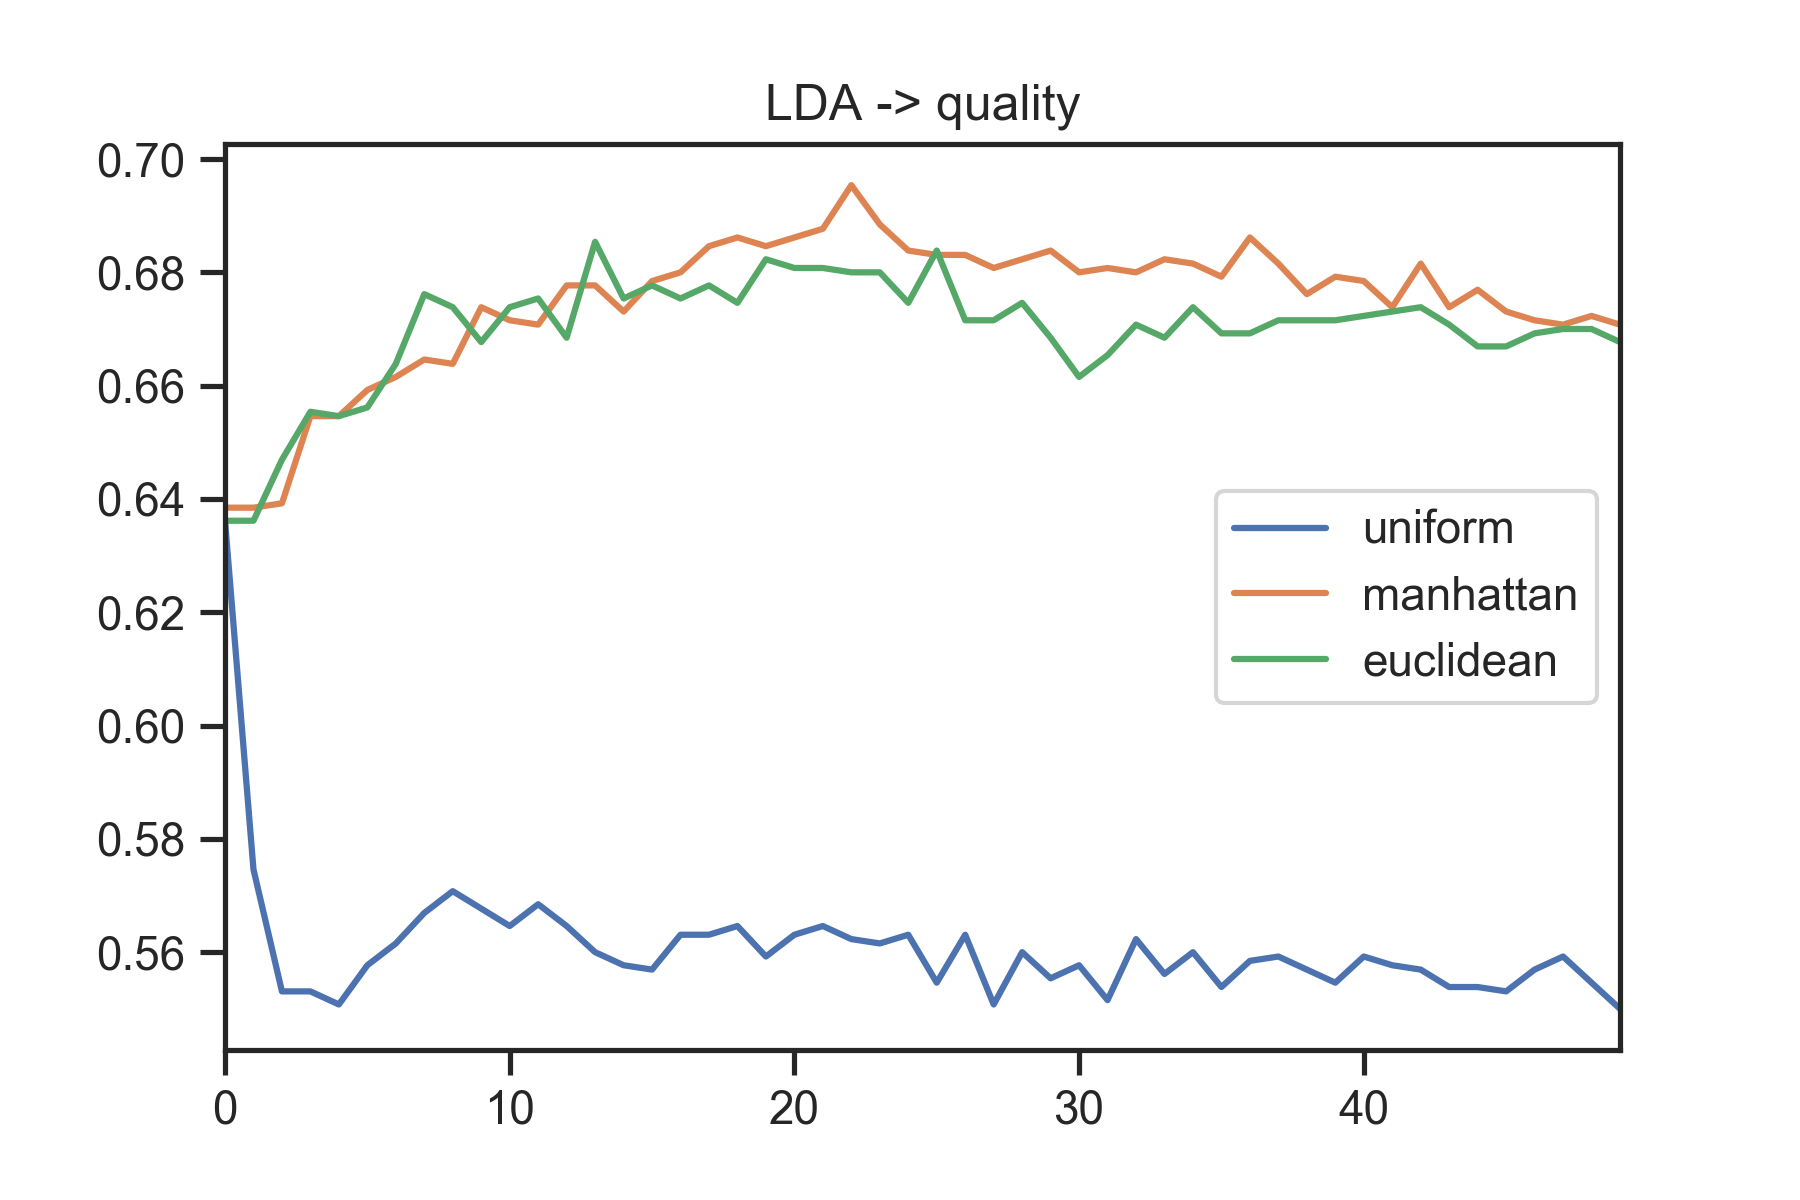
\includegraphics[width=0.48\textwidth]{../plots/Q1_LDA_quality.png}}
\end{figure}
\noindent
\textbf{Some discussion on the relationship between the features from any analysis you performed.}\\
KNN can classify two colors really good using no matter uniform, manhattan or euclidean or k values from 1 to 50. Although the accuracy rate fluctuates, it is mainly above 99 percent, with using some parameters slightly better than using others. And if we change a random state value, the whole situation could change. And this is also true for our four selected features, they work slightly better than using all features only under some random state value.\\
However, a proper weight, selected features and k value are critical for classifying wine quality. A uniform weight only works as good as other 2 when k=1, and the performance drops sharply as k increases.\\
Splitting data into two colors is comparatively easy, therefore extra features will not make the model overfit, but they will when we classify quality, since quality has a more complex relationship with other features.\\\\ 
\textbf{Compare Performance Differences between PCA and LDA. Did either of these methods help in this situation? Which worked better for the task? Did normalization impact the performance of either of them?}\\
Generally, LDA performs slightly better than PCA. And using distance weight is better than using uniform weight except when using LDA to predict color, in which uniform weight is the best. Both of PCA and LDA make no contribution to increasing the accuracy. They only reduce the number of variables. As shown below, PCA is sensitive to unscaled data while LDA is not affected by data normalization. Let $H$ be a centering matrix and $v$ be an eigenvector before data normalization. For LDA, the original solution is $S_Bv=\lambda S_Wv$, by multiplying $H$ on the left and $HH^{-1}$ on the right we get $HS_BHH^{-1}v=\lambda HS_WHH^{-1}v$, which is equivalent to $S_{Bnew}H^{-1}v=\lambda S_{Wnew}H^{-1}v$, which means $H^{-1}v$ is the new eigenvector with the same eigenvalue $\lambda$. Hence, LDA is not affected by data normalization. However, for PCA, the solution is $Sv=\lambda v$, multiplying an $H$ will change its result.
\begin{figure}[H]
\captionsetup[subfigure]{labelformat=empty}
\centering
\subfloat[]{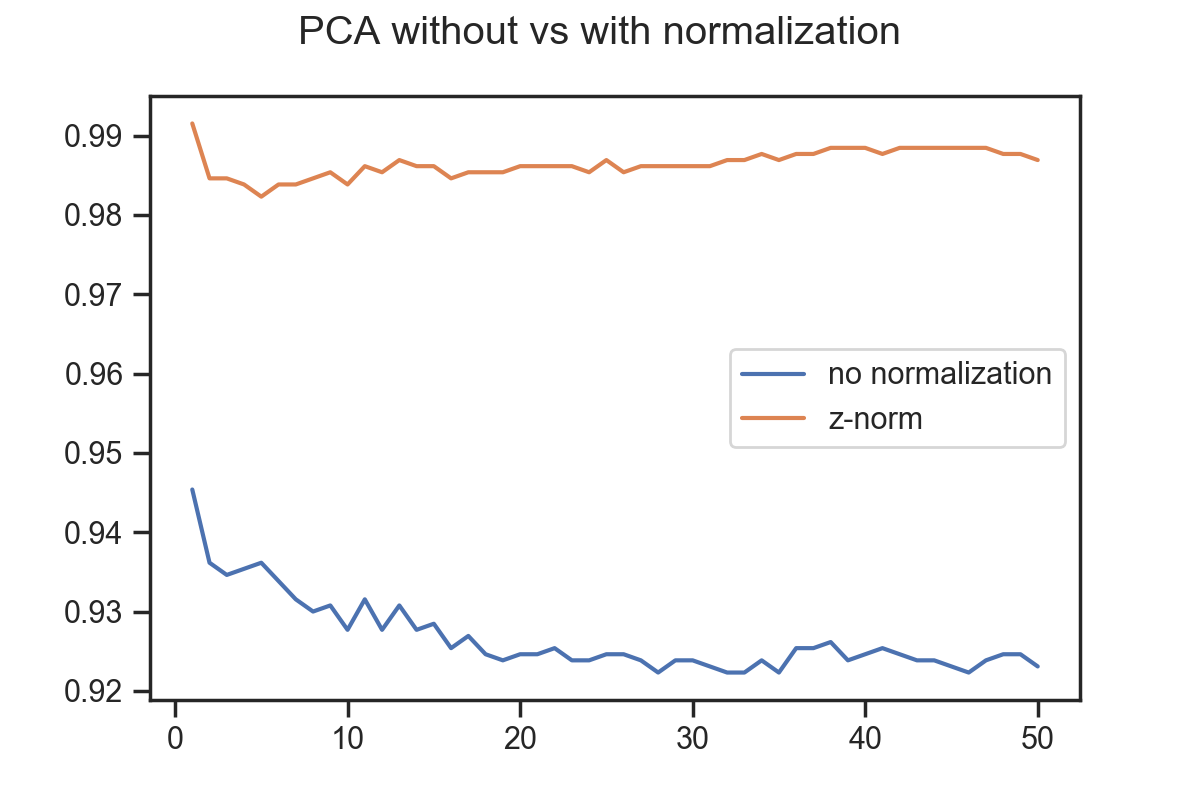
\includegraphics[width=0.48\textwidth]{../plots/Q1_PCA_ifNormalized}}
\subfloat[] {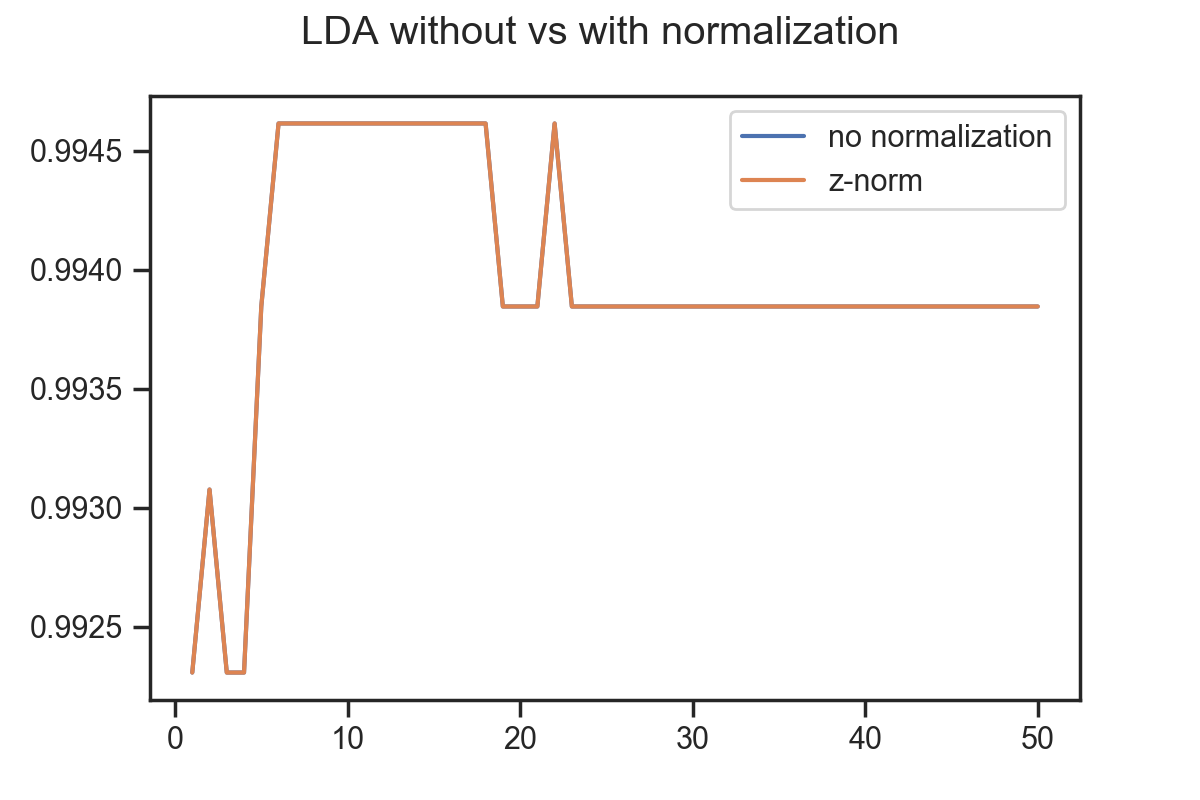
\includegraphics[width=0.48\textwidth]{../plots/Q1_LDA_ifNormalized.png}}
\end{figure}
\noindent
\textbf{Scatter Plots of PCA and LDA}
\begin{figure}[H]
\captionsetup[subfigure]{labelformat=empty}
\centering
\subfloat[]{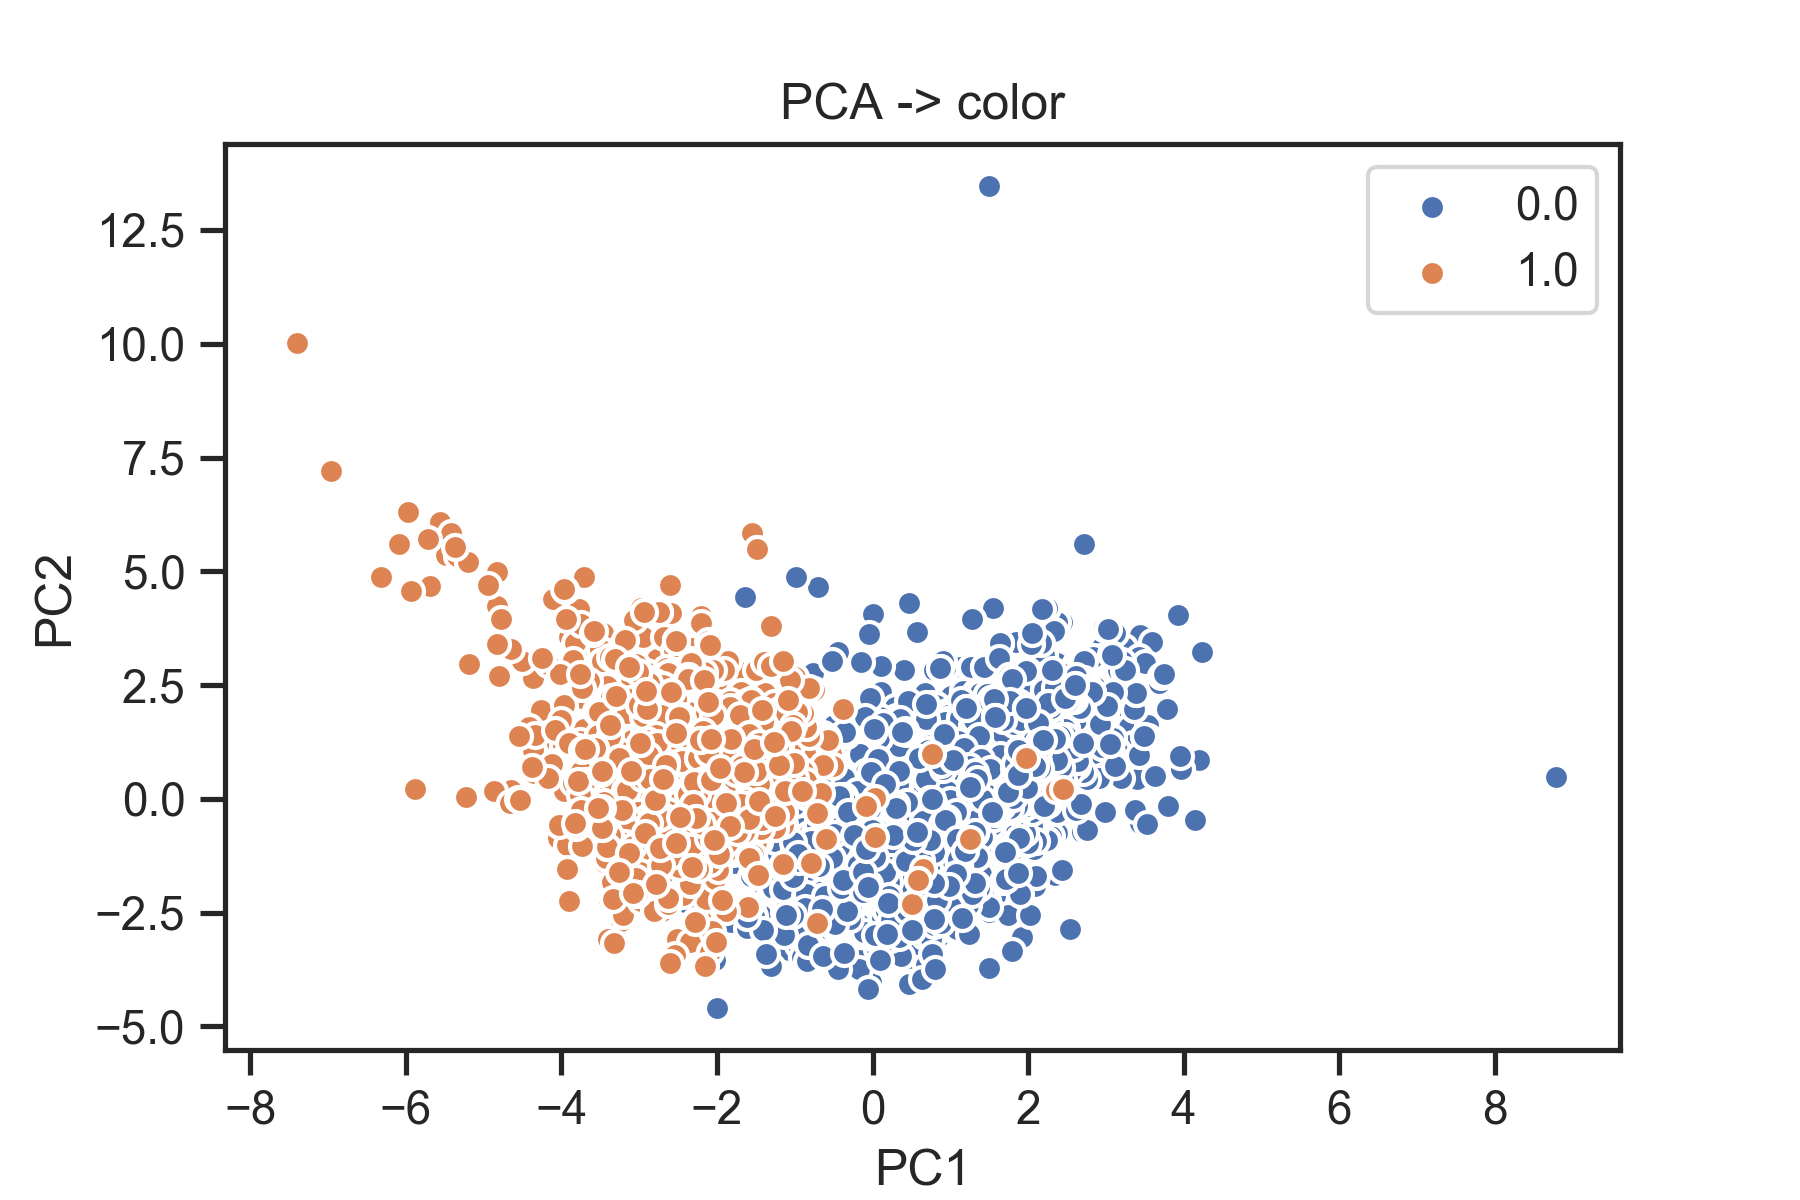
\includegraphics[width=0.48\textwidth]{../plots/Q1_PCA_Scatter_color.png}}
\subfloat[] {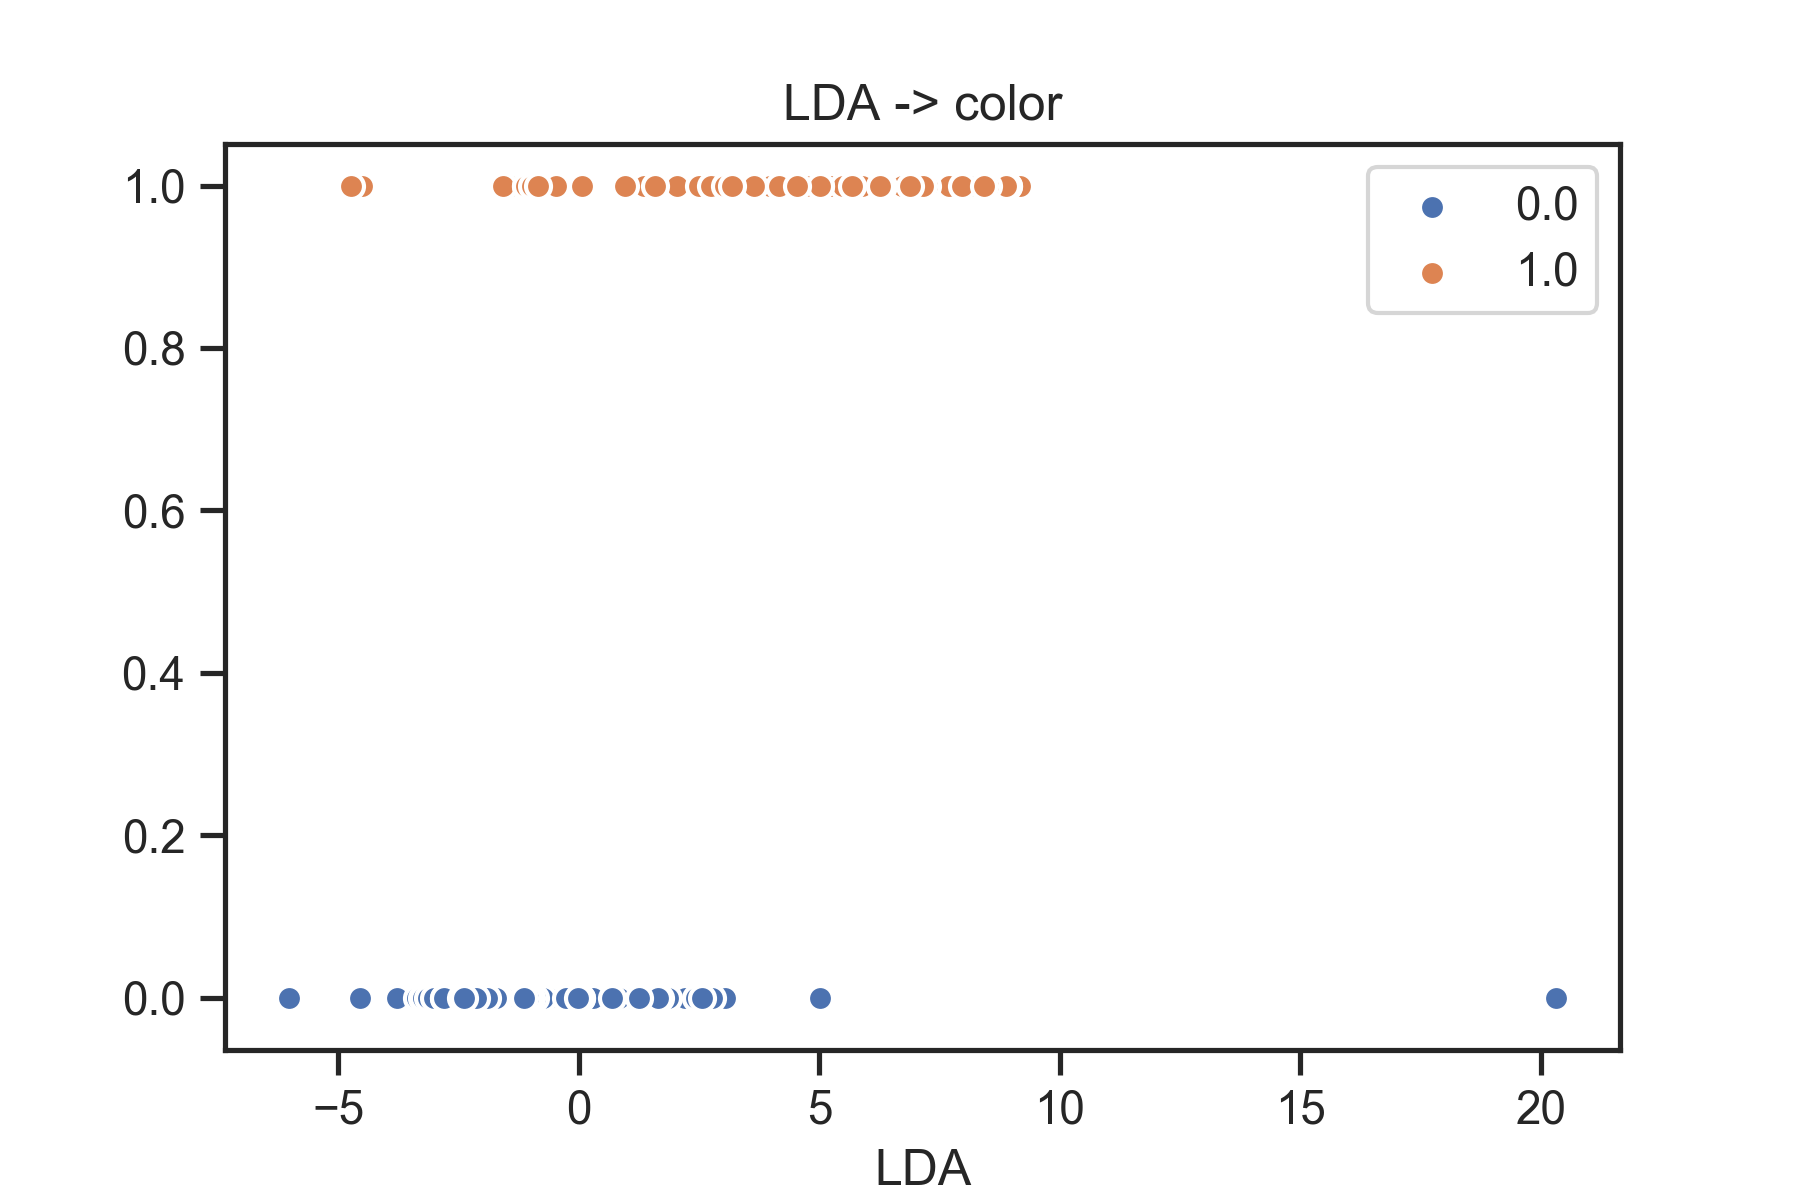
\includegraphics[width=0.48\textwidth]{../plots/Q1_LDA_Scatter_color.png}}
\end{figure}
% \vspace*{-2.0cm}
\begin{figure}[H]
\captionsetup[subfigure]{labelformat=empty}
\centering
\subfloat[]{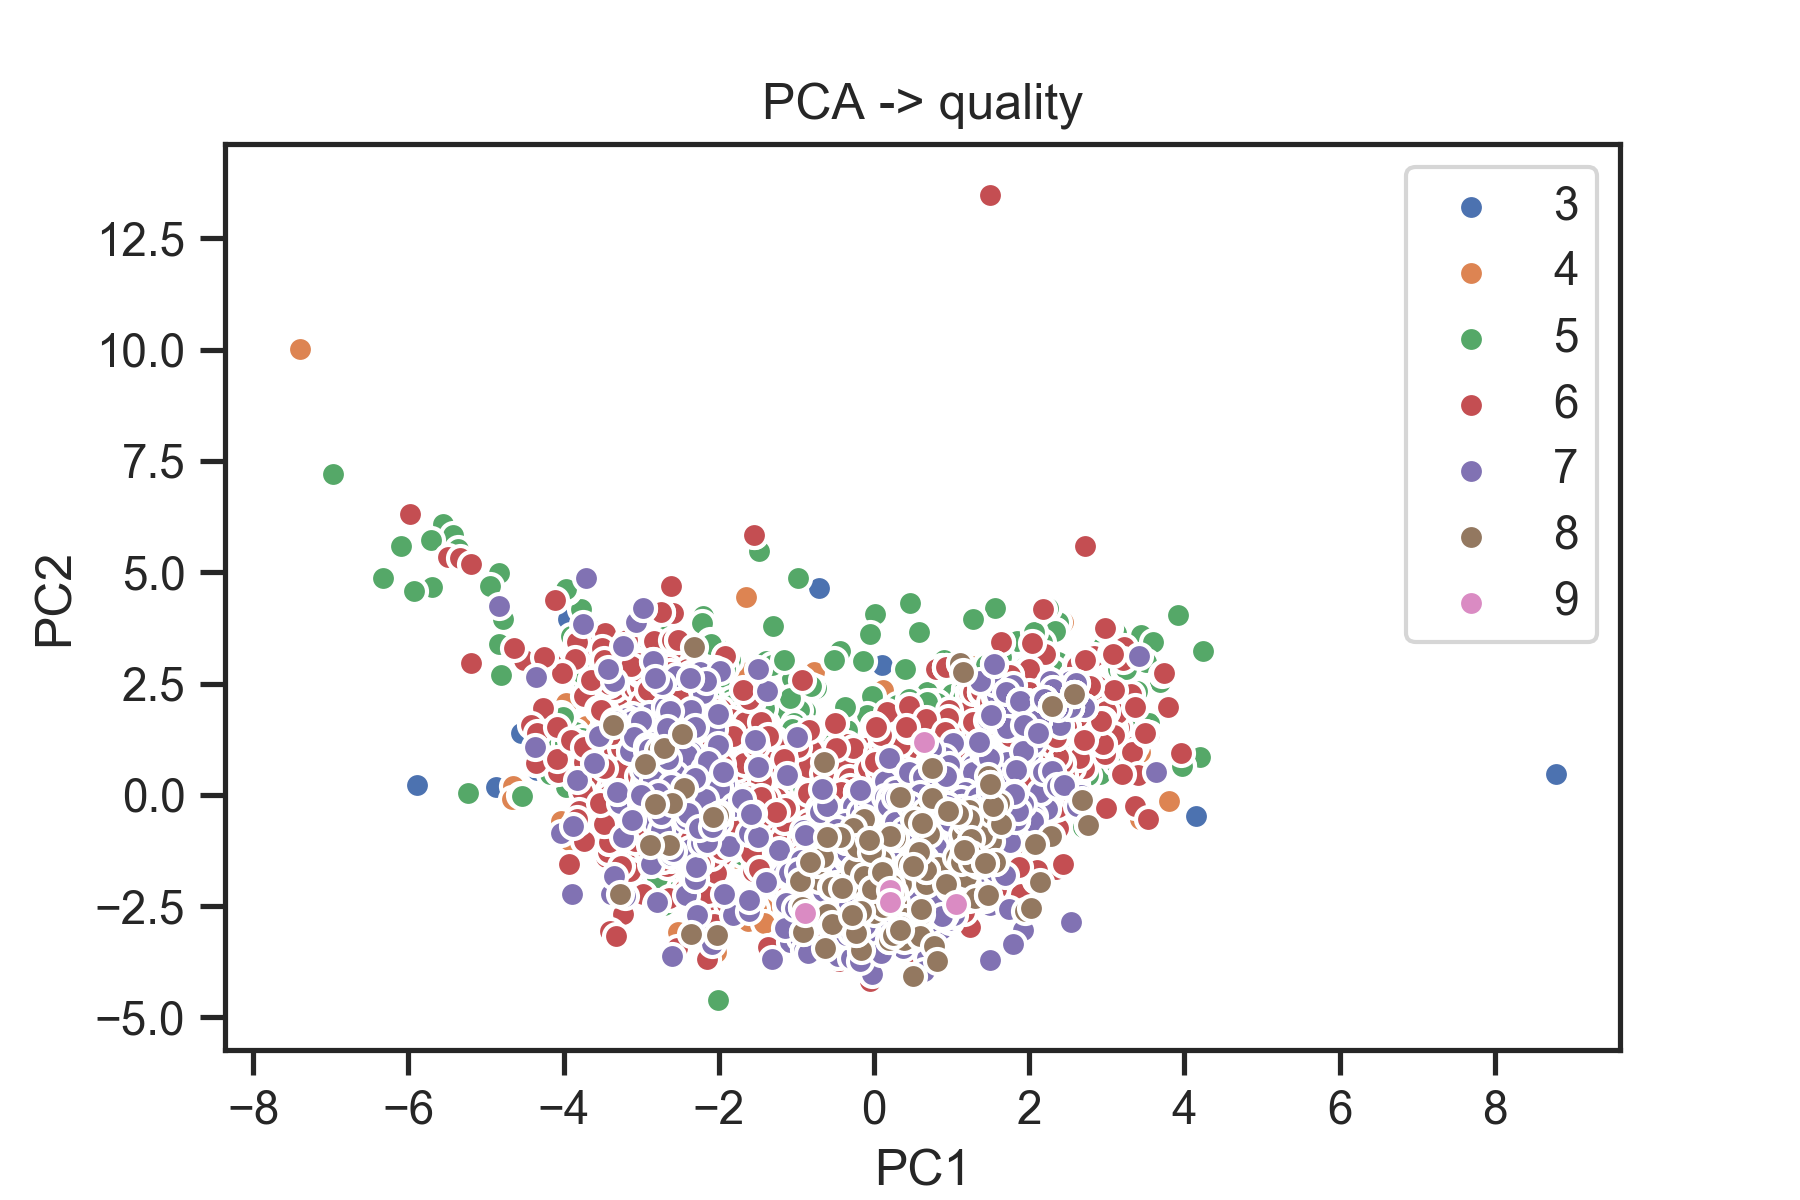
\includegraphics[width=0.48\textwidth]{../plots/Q1_PCA_Scatter_quality.png}}
\subfloat[] {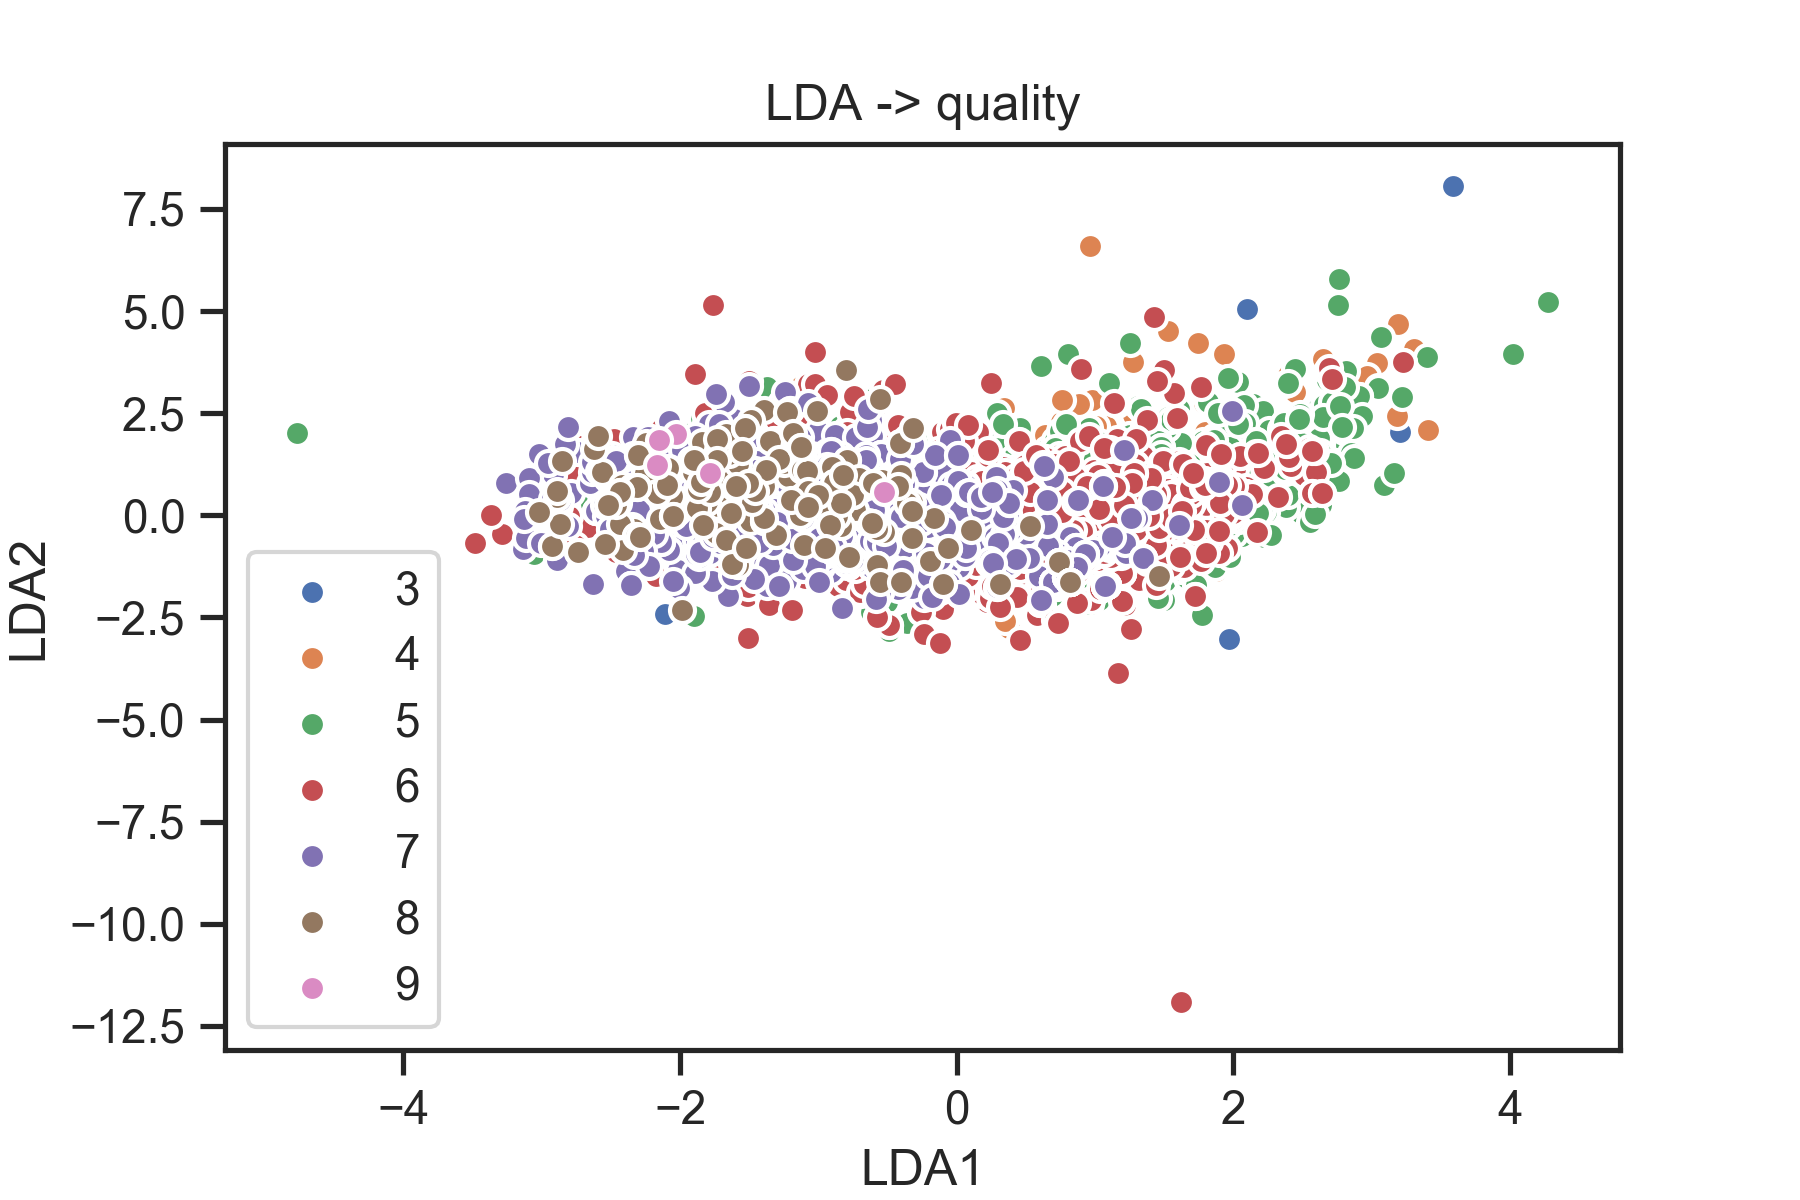
\includegraphics[width=0.48\textwidth]{../plots/Q1_LDA_Scatter_quality.png}}
\end{figure}
\noindent
\textbf{How does this compare or inform your understanding of the data from the pairplots or other results?}\\
Since there are only two colors, we can only plot a 1-dimension graph for LDA. And to deal with the overlap, we draw all label 0 on $y=0$ and all label 1 on $y=1$. Two principle components split two colors clearly, while there is huge overlap between two colors in the 1D graph in LDA. But we cannot compare a 1D graph to a 2D graph so we cannot say PCA is better than LDA. Both algorithms perform poorly on predicting the quality using only two components, as all points are mixed together. The scatter of each class in LDA plot is closer than PCA because LDA minimize the within class variance.
\end{document}